\documentclass[a4paper]{report}

\usepackage{graphicx}
\usepackage{float}
\usepackage{hyperref}
\usepackage{xcolor}
\usepackage[spanish]{babel}
\usepackage{listings}
\usepackage{enumitem}
\usepackage[utf8]{inputenc}
\usepackage{pdfpages}
\usepackage{graphics}

\lstset{language=c, frame=tlrb, basicstyle=\scriptsize, breaklines=true, numberbychapter=false,numbers=left}
\setlist[enumerate]{noitemsep}
\setlist[itemize]{noitemsep}

\bibliographystyle{unsrt}

\renewcommand{\lstlistingname}{Listado}
\renewcommand*{\lstlistlistingname}{Índice de Listados}

\begin{document}

\setlength{\parindent}{0cm}
\renewcommand{\tablename}{Tabla}

\title{Universidad Nacional de La Plata\\Facultad de Informática\\ \bigskip
{\large Tesis presentada para obtener el grado de \\}  Magister en Cómputo de Altas Prestaciones\\ \bigskip
  Infraestructura para el Análisis de Rendimiento}

\author{
  Alumno: Andrés More - {\tt amore@hal.famaf.unc.edu.ar}\\
  Director: Dr Fernando G. Tinetti - {\tt fernando@lidi.info.unlp.edu.ar}
}

\date{Abril de 2015}

\maketitle

\begin{abstract}

En el área del cómputo de altas prestaciones las aplicaciones son construidas por especialistas del dominio del problema, no siempre expertos en optimización de rendimiento. Se identifica entonces la necesidad de un método sistemático y automático para soportar el análisis de rendimiento.

\bigskip

Este trabajo revisa la construcción de una infraestructura que simplifica el análisis de rendimiento; incluyendo su aplicación mediante casos de estudio como etapa de validación. El objetivo es facilitar la tarea evitando la tediosa recolección de datos relevantes de modo manual, permitiendo más tiempo de experimentación para la optimización propiamente dicha.

\bigskip

La infrastructura brinda información de contexto sobre un programa y el sistema donde se ejecuta. Esto incluye su comportamiento al incrementar las únidades de cómputo o el tamaño del problema,
el perfil de ejecución, sus cuellos de botella y la utilización de los recursos disponibles.

\bigskip

En particular, este trabajo contribuye entonces con un generador automático de reportes de rendimiento para aplicaciones de cómputo de altas prestaciones utilizando tecnología {\it OpenMP} sobre sistemas {\it GNU/Linux}.

\end{abstract}

\tableofcontents

\listoffigures
\listoftables
\lstlistoflistings

\chapter{Introducción}

Este capítulo introduce el tema bajo estudio, definiendo los objetivos principales, las contribuciones logradas durante la investigación, y detallando la estructura del resto del documento.

\section{Motivación}

En el área de cómputo de altas prestaciones (o {\it HPC}, por las siglas en inglés de {\it High Performance Computing}) los desarrolladores son los mismos especialistas del dominio del
 problema a resolver. Las rutinas más demandantes de cálculo son en su mayoría científicas y su gran complejidad hace posible su correcta implementación sólo por los mismos investigadores.
Estas cuestiones resultan en un tiempo reducido de análisis de resultados e impactan directamente en la productividad de los grupos de investigación y desarrollo.

\bigskip

Con mayor impacto que en otras áreas de la computación, el código optimizado correctamente puede ejecutarse órdenes de magnitud mejor que una implementación directa \cite{mm-tool}. 
Esto implica que invertir en optimización de un programa puede tener un retorno interesante a largo plazo si las simulaciones a realizar son demasiadas.

\bigskip

Se suele utiliza programación en paralelo para obtener una mejor utilización de la capacidad de cómputo disponible; aumentando por lo tanto la complejidad de implementación, depuración y
optimización con la que el experto en el dominio necesita trabajar en el día a día \cite{is-parallel-programming-hard}.

\bigskip

Frecuentemente el proceso de optimización termina siendo hecho de modo {\it ad-hoc}, sin conocimiento pleno de las herramientas disponibles y sus capacidades, y sin la utilización de
información cuantitativa para dirigir los esfuerzos de optimización. Es incluso frecuente la implementación directa de algoritmos en lugar de la utilización de librerías ya disponibles,
optimizadas profundamente y con correctitud garantizada \cite{mklbook}.

\section{Objetivos}

La propuesta principal consiste en el desarrollo de una infraestructura de soporte para el análisis de aplicaciones de cómputo de altas prestaciones.
Este trabajo se realiza como extensión al trabajo final {\it Herramientas para el Soporte de Análisis de Rendimiento} de la Especialización en Cómputo de Altas Prestaciones y Tecnología Grid.

\bigskip

El problema a resolver es simplificar la compleja tarea de realizar un análisis de rendimiento sobre programas de simulación y cálculo científico. El análisis implica la ejecución repetitiva
de varios casos de prueba bajo diferentes condiciones, además de la aplicación de múltiples herramientas para analizar el comportamiento y la utilización de los recursos disponibles.

\bigskip

La infraestructura desarrollada implementa un procedimiento de análisis de rendimiento ejecutando pruebas de referencia, herramientas de perfil de rendimiento y graficación de resultados.
La infraestructura genera como etapa final un informe detallado que soporta la tarea de optimización con información cuantitativa.
El reporte final incluye datos estadísticos de la aplicación y el sistema donde se ejecuta, además de gráficos de desviación de resultados, escalamiento de problema y cómputo, e identificación
de cuellos de botella.

\section{Contribuciones}

La siguiente lista enumera las diferentes publicaciones realizadas durante el cursado del magister y el desarrollo de la tesis.

\begin{enumerate}
\item Estudio de Multiplicación de Matrices. Reporte Técnico. Realizado como parte del curso {\it Programación en Clusters} dictado por el Dr {\it Fernando Tinetti} \cite{mm-tool}.
\item Artículo {\it Optimizing Latency in Beowulf Clusters}. HPC Latam 2012 \cite{latency}.
\item Comparación de Implementaciones de una Operación BLAS. Reporte técnico realizado como parte del curso {\it Programación GPU de Propósito General} dictado por la Dra {\it Margarita Amor}.
\item Sección {\it Intel Cluster Ready} e {\it Intel Cluster Checker} en el libro {\it Programming Intel Xeon Phi}. Intel Press. 2013 \cite{xeonphi}.
\item Reseña del Libro {\it Intel Xeon Phi Coprocessor High Performance Programming} - JCS\&T Vol 13 N 2 Octubre 2013 \footnote{\href{http://journal.info.unlp.edu.ar/journal/journal36/papers/JCST-Oct13-BR1.pdf}{JCS\&T Vol. 13 No. 2}}.
\item Artículo {\it Lessons Learned from Contrasting BLAS Kernel Implementations} - XIII Workshop Procesamiento Distribuido y Paralelo (WPDP), 2013 \cite{lessons}.
\end{enumerate}

Las publicaciones realizadas pueden encontrarse en el apéndice \ref{contributions}.

\section{Metodología}

En base al problema y a los objetivos establecidos previamente, la metodología adoptada es la siguiente:

\begin{enumerate}
\item Analizar el estado del arte del análisis de rendimiento y las herramientas utilizadas para ello.
\item Formular la solución específica necesaria para simplificar la tarea.
\item Identificar que tipos de gráficos y tablas pueden resumir la información obtenida de modo de facilitar su utilización.
\item Dada una propuesta de procedimiento sistemático de análisis de rendimiento, automatizarlo y analizar potenciales mejoras de utilidad.
\item Aplicar la infraestructura sobre núcleos de cómputo conocidos para poder focalizar los esfuerzos en la mejora del reporte.
\item Documentación de la experiencia
\end{enumerate}

\section{Estructura}

El resto del documento se estructura de la siguiente manera:

\begin{itemize}
\item Capitulo \ref{Estado del Arte}: revisa el estado del arte de los temas incluídos dentro del análisis de rendimiento: paralelismo, leyes fundamentales, métricas, técnicas de análisis,
herramientas de soporte y pruebas de rendimiento.
\item Capitulo \ref{Descripcion del Problema}: describe la cuestión a resolver como parte de esta tesis. Los problemas usuales del propio análisis, métodos de optimización a soportar, y una
discusión de como debería ser una infrastructura de soporte.
\item Capitulo \ref{Propuesta de Solucion}: muestra la propuesta de solución. El procedimiento general propuesto, los comandos a utilizar, y la arquitectura y diseño de la solución implementada junto con una descripción de las diferentes secciones generadas por la herramienta en el reporte final.
\item Capitulo \ref{Casos de Aplicacion}: aplica la solución a casos de estudio. Se incluyen los resultados de tres ejemplos.
\item Capítulo \ref{Conclusiones y Trabajo Futuro}: concluye reflejando los objetivos y proponiendo líneas de trabajo futuro. 
\item Apéndice \ref{examples}: muestra los reportes completos de los casos de aplicación.
\item Apéndice \ref{contributions}: contiene las publicaciones realizadas durante el transcurso de la carrera.

\end{itemize}

\chapter{Estado del Arte} \label{Estado del Arte}

Este capítulo revisa el estado del arte de los temas relevantes a este trabajo.

\section{Análisis de Rendimiento}\label{chapter:analysis}

Esta sección introduce el concepto de rendimiento y teoría básica sobre su análisis; además revisa las herramientas disponibles para ello.

\subsection{Definición}

El rendimiento se caracteriza por la cantidad de trabajo de cómputo que se logra en comparación con la cantidad de tiempo y los recursos ocupados.
El rendimiento debe ser evaluado entonces de forma cuantificable, utilizando alguna métrica en particular de modo de poder comparar relativamente dos sistemas o
el comportamiento de un mismo sistema bajo una configuración distinta.

\subsection{Paralelismo}

Una vez obtenida una implementación eficiente, la única alternativa para mejorar el rendimiento es explotar el paralelismo que ofrecen los sistemas de cómputo.
Este paralelismo se puede explotar a diferentes niveles, desde instrucciones especiales que ejecutan sobre varios datos a la vez (vectorización),
hasta la utilización de múltiples sistemas para distribuir el trabajo.

\bigskip

El cálculo de las mejoras posibles de rendimiento, cómo priorizarlas y la estimación de su límite máximo es una tarea compleja. 
Para ello existen algunas leyes fundamentales utilizadas durante el análisis de rendimiento.

\subsubsection{Ley de {\it Amdahl}}

 La ley de {\it Amdahl} \cite{amdahl} dimensiona la mejora que puede obtenerse en un sistema de acuerdo a las mejoras logradas en sus componentes. 
Nos ayuda a establecer un límite máximo de mejora y a estimar cuales pueden ser los resultados de una optimización.

\bigskip

La mejora de un programa utilizando cómputo paralelo está limitada por el tiempo necesario para completar su fracción serial o secuencial. En la mayoría de los casos, el paralelismo sólo impacta notoriamente cuando es utilizado en un pequeño número de procesadores, o cuando se aplica a problemas altamente escalables (denominados {\it Embarrassingly Parallel Problems} en inglés). Una vez paralelizado un programa, los esfuerzos suelen ser enfocados en cómo minimizar la parte secuencial, algunas veces haciendo más trabajo redundante pero en forma paralela.

\bigskip

Suponiendo que una aplicación requiere de un trabajo serial más un trabajo paralelizable, la ley de {\it Amdahl} calcula la ganancia ($ S $) mediante la Ecuación \ref{eq:amdahl}.
Donde $ P $ es el porcentaje de trabajo hecho en paralelo, ($ 1-P $) es entonces el trabajo en serie o secuencial, y $ N $ la cantidad de unidades de cómputo a utilizar.

\begin{eqnarray}
\label{eq:amdahl}
S = \frac{1}{(1 - P) + \frac{P}{N}}
\end{eqnarray}

Esta ley establece que incluso teniendo infinitas unidades de cómputo la ganancia está limitada.
La Tabla \ref{fig:amdahl} muestra que no importa la cantidad de unidades de procesamiento que sean utilizadas, siempre existe un límite en la práctica.

\begin{table}[H]
\caption{Mejora Máxima según {\it Amdahl}}
\centering
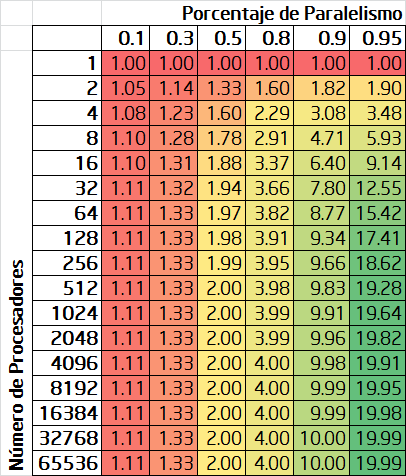
\includegraphics[width=7cm]{amdahl.png}

\label{fig:amdahl}
\end{table}

Por ejemplo, en el caso de tener sólo un $ 10\% $ de paralelismo en una aplicación, la mejora nunca va a superar $ 1.1 $ veces la original.
En el caso de tener un $ 95\% $ de paralelismo, la mejora no puede ser mayor a $ 20 $ veces la original.

\bigskip

En el caso de conocer los tiempos de ejecución para distinto número de procesadores, la porción serial/paralelo puede ser aproximada.

\subsubsection{Ley de {\it Gustafson}}

Desde un punto de vista más general, la ley de {\it Gustafson} \cite{gustafson} (Ecuación \ref{eq:gustafson}) establece que las aplicaciones que manejan problemas
repetitivos con conjuntos de datos similares pueden ser fácilmente paralelizadas. En comparación, la ley anterior no escala el tamaño o
resolución de problema cuando se incrementa la potencia de cálculo, es decir asume un tamaño de problema fijo. 

\begin{eqnarray}
\label{eq:gustafson}
Speedup(P) = P - \alpha \times (P - 1)
\end{eqnarray}

donde $ P $ es el número de unidades de cómputo y $ \alpha $ el porcentaje de trabajo paralelizable.

\bigskip

Al aplicar esta ley obtenemos que un problema con datos grandes o repetitivos en cantidades grandes puede ser computado en paralelo muy eficientemente.
Nos es útil para determinar el tamaño de problema a utilizar cuando los recursos de cómputo son incrementados. 
En el mismo tiempo de ejecución, el programa resuelve entonces problemas más grandes.

\begin{table}[H]
\caption{Mejora Máxima según {\it Gustafson}}
\centering
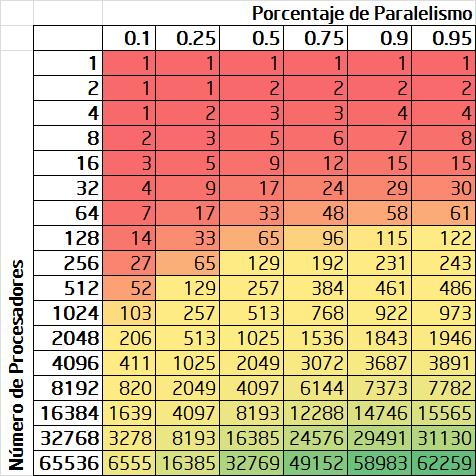
\includegraphics[width=7cm]{gustafson.png}
\label{fig:gustafson}
\end{table}

Similarmente al cuadro anterior, podemos deducir de la Tabla \ref{fig:gustafson} que en el caso de un programa con sólo $ 10\% $ de paralelismo, al incrementar los recursos $ 64 $ veces sólo podemos incrementar el tamaño del problema $ 7 $ veces. En el otro extremo, nos estima un incremento de $ 61 $ veces en el caso de tener $ 95\% $ de paralelismo.

\subsubsection{Métrica de {\it Karp-Flatt}}

Esta métrica es utilizada para medir el grado de paralelismo de una aplicación \cite{karp-flatt}. 
Su valor nos permite rápidamente dimensionar la mejora posible al aplicar un alto nivel de paralelismo.

\bigskip

Dado un cómputo paralelo con una mejora de rendimiento $ \psi $ en $ P $ procesadores, donde $ P > 1 $. 
La fracción serial {\it Karp-Flatt} representada con $ e $ y calculada según la Ecuación \ref{eq:karp-flatt} es determinada experimentalmente, 
mientras menor sea $ e $ mayor se supone el nivel de paralelismo posible.

\begin{eqnarray}
\label{eq:karp-flatt}
 e = \frac{\frac{1}{\psi} - \frac{1}{p}}{1 - \frac{1}{p}} 
\end{eqnarray}

Para un problema de tamaño fijo, la eficiencia típicamente disminuye cuando el número de procesadores aumenta. 
Se puede entonces proceder a determinar si esta disminución es debida a un paralelismo limitado, a un algoritmo no optimizado o un problema de arquitectura del sistema.

\subsection{Métricas}

Algunos ejemplos de métricas de rendimiento son:

\begin{enumerate}
\item El ancho de banda y la latencia mínima de un canal de comunicación,
  una jerarquía de memorias o de una unidad de almacenamiento.
\item La cantidad de instrucciones, operaciones, datos o trabajo procesado
  por cierta unidad de tiempo.
\item El rendimiento asociado al costo del equipamiento, incluyendo mantenimiento
 periódico, personal dedicado y gastos propios del uso cotidiano.
\item El rendimiento por unidad de energía consumida (electricidad).

\end{enumerate}

Un método de medición de rendimiento indirecto consiste en medir el uso de los recursos del sistema mientras se ejercita el mismo con un trabajo dado.
Por ejemplo: el nivel de carga de trabajo en el sistema, la cantidad de operaciones realizadas por el sistema operativo o la unidad de procesamiento, la utilización de memoria o
archivos temporales e incluso el ancho de banda de red utilizado durante la comunicación.

\subsection{Técnicas de Análisis}

El procedimiento de mejora general usualmente consiste en ciclos iterativos de medir, localizar, optimizar y comparar (Figura \ref{fig:cycle}). 
Es muy importante mantener la disciplina en realizar un cambio a la vez ya que esto asegura resultados reproducibles y convergentes, sin efectos no deseados.

\begin{figure}[H]
\begin{center}
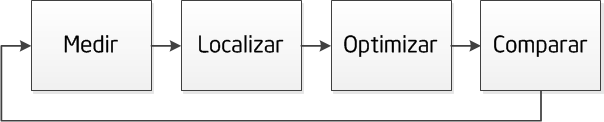
\includegraphics[width=10cm]{cycle.png}
\caption{Optimización Iterativa}
\label{fig:cycle}
\end{center}
\end{figure}

A la hora de tomar decisiones, éstas deben estar basadas en datos concretos, ya que en caso contrario se podría estar trabajando sin llegar a obtener un rédito adecuado.

\bigskip

En el caso de tener problemas de desviación en los resultados medidos, es aconsejable obtener un gran número de muestras y utilizar un valor promedio para asegurarse de evitar errores de
medición tanto como sea posible. También es preferible aumentar el tamaño del problema a resolver, o la definición de los resultados, para ejercitar por más tiempo y tener así un resultado 
más estable.
Suponiendo una distribución normal de resultados, se suele controlar que haya menos de 3 desviaciones estandar de diferencia. 
Se busca que la mayoría de los resultados queden cerca de su promedio, como muestra la Figura \ref{fig:deviation}.

\begin{figure}[H]
\centering
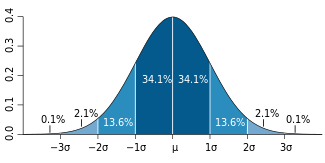
\includegraphics[width=8cm]{deviation.png}
\caption{Desviación en una distribución normal [Wikipedia]}
\label{fig:deviation}
\end{figure}

Los resultados deben también ser correctamente guardados para evitar problemas de datos. Si la configuración del sistema es dinámica entonces la
reproducción de resultados es no trivial. En el caso de no tener una configuración de sistema estable en el tiempo, es recomendable siempre
ejecutar una versión optimizada contra una versión de referencia en un mismo sistema de cómputo.

\bigskip

Para comparar es recomendable utilizar la media geométrica según la Ecuación \ref{eq:geomean} en lugar de la aritmética \cite{how-not-to-lie}, ya que permite dimensionar la tendencia central de un valor típico en un conjunto de números. Esto permite reducir el impacto de ruido introducido por una ejecución problemática.

\begin{equation}
\label{eq:geomean}
G = \sqrt[n]{x_{1} \ldots x_{n}}
\end{equation}

La raíz n-ésima de un número (para un $ n $ posiblemente muy grande), es una operación ineficiente ya que se implementa con métodos numéricos de aproximación siguiendo el método de {\it Newton} \cite{numerical-analysis}. En cambio se suele tomar el anti-logaritmo del promedio de los logaritmos de los valores siguiendo la ecuación \ref{eq:geomean-log}.

\begin{equation}
\label{eq:geomean-log}
G = 10 ^{( log _{10} (x_{1}) + \ldots + log _{10} (x_{n}) ) / n}
\end{equation}

\subsection{Trabajos Relacionados}

Al ser un tema que es relevante en toda disciplina que realice simulaciones computarizadas, existen innumerables trabajos relacionados.
Una introducción puede ser consultada en \cite{intro}. Una revisión general en \cite{overview}. Una propuesta de hacia donde va el estado del arte en \cite{future}. Patrones útiles para ser reusados en \cite{patterns}. Como capturar la información necesaria en \cite{capturing}. Un esfuerzo de optimización automática en \cite{automatic}. Más detalles del estado del arte del análisis del rendimiento en Cómputo de Altas Prestaciones en \cite{hybrid}.

\section{Herramientas}

Actualmente existen numerosas y diversas herramientas para el análisis de rendimiento \cite{gregg}. Estas funcionan a diferentes niveles de abstracción: desde contadores de eventos a nivel de {\it hardware}, pasando por monitores de recursos dentro del núcleo del sistema operativo, instrumentación de código, y hasta la simple utilización del tiempo de ejecución de una aplicación o la comparación contra un trabajo similar de referencia. 

\subsection{Pruebas de Rendimiento}

Para medir el rendimiento se utilizan pruebas de referencia (en inglés, {\em benchmarks}); éstas pueden ser aplicaciones sintéticas construidas específicamente, o bien aplicaciones del mundo real computando un problema prefijado. Al tener valores de referencia se pueden caracterizar los sistemas de modo de predecir el rendimiento de una aplicación.
Los valores a los que se llegan con un {\it benchmark} suelen ser más prácticos y comparables que los teóricos de acuerdo a condiciones ideales de uso de recursos.
También es posible garantizar que el sistema sigue en un mismo estado con el correr del tiempo y después de cambios de configuraciones en {\it hardware} o {\it software}.

\bigskip

Las características deseables en un {\it benchmark} son portabilidad, simplicidad, estabilidad y reproducción de resultados. Esto permite que sean utilizadas para realizar
mediciones cuantitativas y así realizar comparaciones de optimizaciones o entre sistemas de cómputo diferentes. También se pide que el tiempo de
ejecución sea razonable y que el tamaño del problema sea ajustable para poder mantener su utilidad con el paso del tiempo y el avance de las tecnologías.

\bigskip

A continuación se introducen algunas de las más utilizadas para cómputo de altas prestaciones (listadas en la tabla \ref{table:benchmark-list}),
y posteriormente algunos detalles específicos e instancias de sus datos de salida para ser utilizados a manera de ejemplo.

\begin{table}[H]
    \caption{Pruebas de Rendimiento}
    \centering
    \begin{tabular}{|l|l|l|}\hline
      {\bf Nombre} & {\bf Componente} & {\bf Descripción} \\ \hline
      STREAM & Memoria & Ancho de banda sostenido \\ \hline
      Linpack & Procesador & Operaciones de punto flotante \\ \hline
      IMB Ping Pong & Red & Latencia/Ancho de banda de red \\ \hline
      HPCC & Sistema & Múltiples componentes \\ \hline
        \end{tabular}
  \label{table:benchmark-list}
\end{table}

\bigskip

Los {\it benchmarks} pueden ser utilizados para diferentes propósitos. Primero, los valores reportados son usados como referencia para contrastar rendimiento.
Segundo, su desviación demuestra que algo ha cambiado en el sistema (por lo tanto su no desviación indica que el sistema sigue saludable). Por último,
un {\it benchmark} sintético implementando el cómputo que uno quiere realizar muestra el rendimiento máximo posible a obtener en la práctica.

\subsubsection{STREAM}

STREAM \cite{stream} es un {\it benchmark} sintético que mide el ancho de banda de memoria sostenido en MB/s y el rendimiento de computación relativa de algunos vectores simples de cálculo. Se utiliza para dimensionar el ancho de banda de acceso de escritura o lectura a la jerarquía de memoria principal del sistema bajo análisis. Dentro de una misma ejecución de este {\it benchmark} se ejercitan diferentes operaciones en memoria, listadas en la tabla \ref{table:stream}.

\begin{table}[H]
\caption{Operaciones del Benchmark STREAM}
  \centering
    \begin{tabular}{|l|l|l|}\hline
      {\bf Función} & {\bf Operación} & {\bf Descripción} \\ \hline
      {\tt copy} & $ \forall i $ $ b_{i} = a_{i} $ & Copia simple \\ \hline
      {\tt scale} & $ \forall i $ $ b_{i} = c \times a_{i} $ & Multiplicación escalar \\ \hline
      {\tt add} & $ \forall i $ $ c_{i} = b_{i} + a_{i} $ & Suma directa \\ \hline
      {\tt triad} & $ \forall i $ $ c_{i} = b_{i} + c \times a_{i} $ & Suma y multiplicación escalar \\ \hline
    \end{tabular} 
 \label{table:stream}
\end{table}

La salida en pantalla muestra entonces los diferentes tiempos conseguidos y la cantidad de información transferida por unidad de tiempo.
Como último paso, el programa valida también la solución computada.

{\small
\begin{verbatim}
  STREAM version $Revision: 1.2 $
  -------------------------------------------------------------
  This system uses 8 bytes per DOUBLE PRECISION word.
  -------------------------------------------------------------
  Array size = 10000000, Offset = 0
  Total memory required = 228.9 MB.
  Each test is run 10 times, but only the *best* time is used.
  -------------------------------------------------------------
  Function     Rate (MB/s)   Avg time     Min time     Max time
  Copy:        4764.1905       0.0337       0.0336       0.0340
  Scale:       4760.2029       0.0338       0.0336       0.0340
  Add:         4993.8631       0.0488       0.0481       0.0503
  Triad:       5051.5778       0.0488       0.0475       0.0500
  -------------------------------------------------------------
  Solution Validates
\end{verbatim}
}

\bigskip

La correcta utilización de la jerarquía de la memoria de un sistema de cómputo es una tarea no trivial \cite{memory}.

\subsubsection{Linpack}

Linpack \cite{linpack} es un conjunto de subrutinas {\it FORTRAN} que resuelven problemas de álgebra lineal como ecuaciones lineales y multiplicación de
matrices. High Performance Linpack (HPL) \cite{hpl} es una versión portable del {\it benchmark} que incluye el paquete Linpack pero modificado para sistemas de memoria distribuida.

\bigskip

Este {\it benchmark} es utilizado mundialmente para la comparación de la velocidad de las supercomputadoras en el ranking TOP500 \footnote{http://www.top500.org/}. 
Un gráfico del TOP500 de los últimos años (Figura \ref{fig:top500}) demuestra claramente la tendencia en crecimiento de rendimiento; también la relación entre el primero,
el último y la suma de todos los sistemas en la lista.

\begin{figure}[H]
\centering
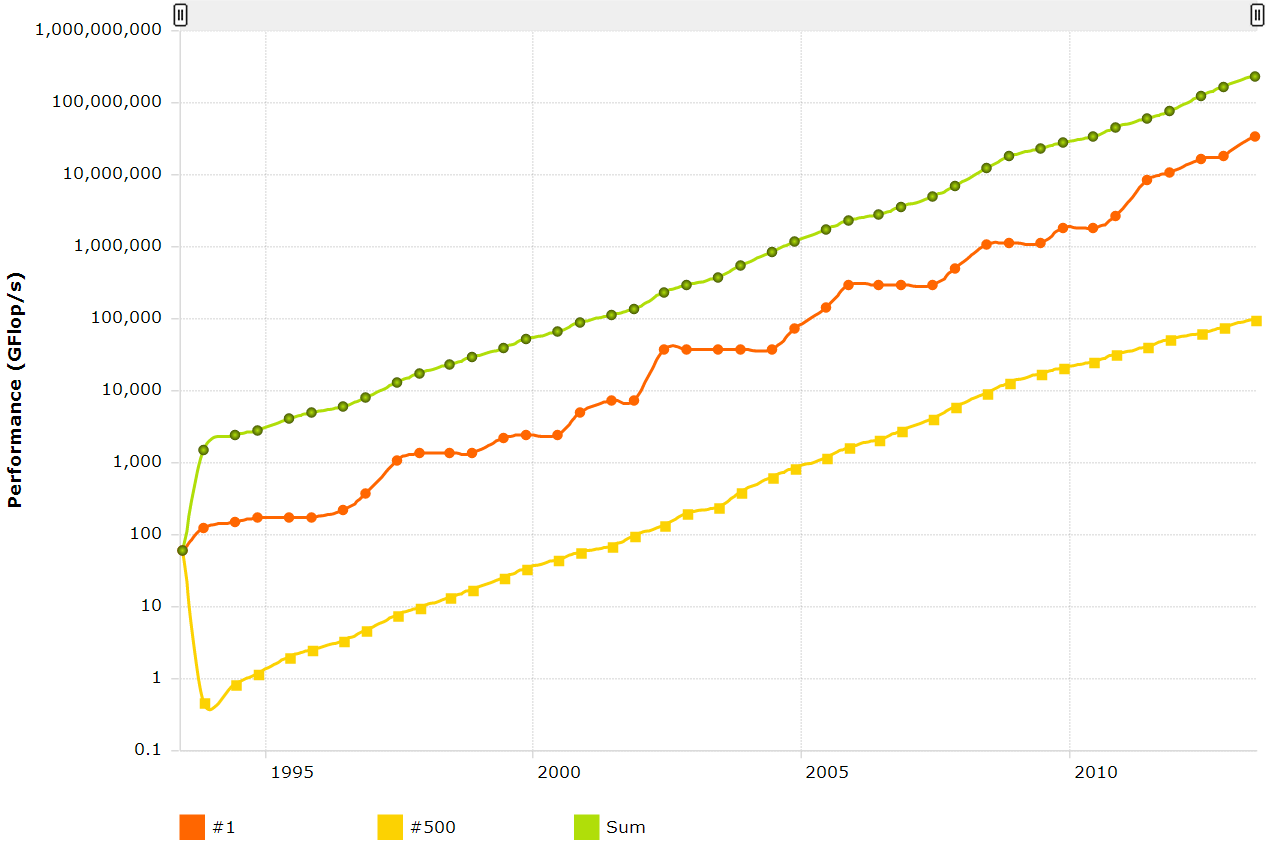
\includegraphics[width=12cm]{top500.png}
\caption{Rendimiento Agregado del Top500 [Top500])}
\label{fig:top500}
\end{figure}

Este {\it benchmark} requiere conocimiento avanzado para una correcta configuración, por ejemplo el tamaño de bloque que se va a utilizar para la distribución de trabajo
debe estar directamente relacionado con el tamaño del {\it cache} de memoria del procesador.

\bigskip

La salida en pantalla resume entonces los datos de entrada y los resultados conseguidos. Como último paso el programa valida que los resultados sean correctos.

{\small
\begin{verbatim}
=================================================================
HPLinpack 2.0 - High-Performance Linpack benchmark - Sep 10, 2008
Written by A. Petitet and R. Clint Whaley
=================================================================
The following parameter values will be used:
N      :   28888
NB     :     168
PMAP   : Row-major process mapping
P      :       4
Q      :       4
PFACT  :   Right
NBMIN  :       4
NDIV   :       2
RFACT  :   Crout
BCAST  :  1ringM
DEPTH  :       0
SWAP   : Mix (threshold = 64)
L1     : transposed form
U      : transposed form
EQUIL  : yes
ALIGN  : 8 double precision words
------------------------------------------------------------------
- The matrix A is randomly generated for each test.
- The relative machine precision (eps) is taken to be 1.110223e-16
- Computational tests pass if scaled residuals are less than 16.0

Column=000168 Fraction=0.005 Mflops=133122.97
...
Column=025872 Fraction=0.895 Mflops=98107.60
======================================================================
T/V                N   NB   P    Q             Time             Gflops
WR01C2R4       28888  168   4    4           165.83          9.693e+01
----------------------------------------------------------------------
||Ax-b||_oo/(eps*(||A||_oo*||x||_oo+||b||_oo)*N) = 0.0043035 .. PASSED
======================================================================
Finished      1 tests with the following results:
1 tests completed and passed residual checks,
0 tests completed and failed residual checks,
0 tests skipped because of illegal input values.
\end{verbatim}
}

\bigskip

Existe cierta controversia de que no es una buena forma de ejercitar un sistema de cómputo distribuido ya que no implica uso significativo de la
red, sólo procesamiento intensivo de aritmética de punto flotante sobre la jerarquía local de memoria.

\subsubsection{Intel MPI Benchmarks}

Es un conjunto de {\it benchmarks} cuyo objetivo es ejercitar las funciones más importantes del estándar para librerías de paso de mensajes
(MPI, por las siglas de {\it Message Passing Interface} en inglés) \cite{mpi-standard}.
El más conocido es el popular ping-pong, el cual ejercita la transmisión de mensajes ida y vuelta entre dos nodos de cómputo con diferentes tamaños de mensajes \cite{latency}.

\bigskip

Para obtener el máximo ancho de banda disponible, se ejercita la comunicación a través de mensajes con datos grandes. 
Para obtener la mínima latencia, se ejercita la comunicación con mensajes vacíos.

{\small
\begin{verbatim}
# Intel (R) MPI Benchmark Suite V3.1, MPI-1 part
# Date                  : Wed Mar  3 10:45:16 2010
# Machine               : x86_64
# System                : Linux
# Release               : 2.6.16.46-0.12-smp
# Version               : #1 SMP Thu May 17 14:00:09 UTC 2007
# MPI Version           : 2.0
# MPI Thread Environment: MPI_THREAD_SINGLE
# Calling sequence was: ../IMB-MPI1 pingpong
# Minimum message length in bytes:   0
# Maximum message length in bytes:   4194304
#
# MPI_Datatype                   :   MPI_BYTE
# MPI_Datatype for reductions    :   MPI_FLOAT
# MPI_Op                         :   MPI_SUM
#
# List of Benchmarks to run: PingPong
#---------------------------------------------------
# Benchmarking PingPong
# #processes = 2
#---------------------------------------------------
#bytes     #repetitions  t[usec]     Mbytes/sec
0              1000           17.13        0.00
1              1000           17.89        0.05
2              1000           17.82        0.11
4              1000           17.95        0.21
...
1048576    40              8993.23    111.19
2097152    20              17919.20  111.61
4194304    10              35766.45  111.84
\end{verbatim}
}

\subsubsection{HPC Challenge}

El {\it benchmark} HPC Challenge \cite{hpcc} (HPCC) está compuesto internamente por un conjunto de varios núcleos de cómputo: entre ellos STREAM, HPL, Ping Pong,
Transformadas de {\it Fourier} y otros más simples ejercitando la red de comunicación.

\bigskip

Este benchmark muestra diferentes resultados que son representativos y puestos en consideración de acuerdo al tipo de aplicación en discusión.
La mejor máquina depende de la aplicación específica a ejecutar, ya que algunas aplicaciones necesitan mejor ancho de banda de memoria, mejor canal de comunicación, o
simplemente la mayor capacidad de cómputo de operaciones flotantes posible.

\bigskip

Una analogía interesante para entender cómo el {\it benchmark} se relaciona con diferentes núcleos de cómputo se muestra en la Figura \ref{fig:locality}. Por ejemplo al tener un problema que utiliza principalmente acceso a memoria local, se puede suponer que un sistema con buenos resultados de STREAM va ser útil.

\begin{figure}[H]
\begin{center}
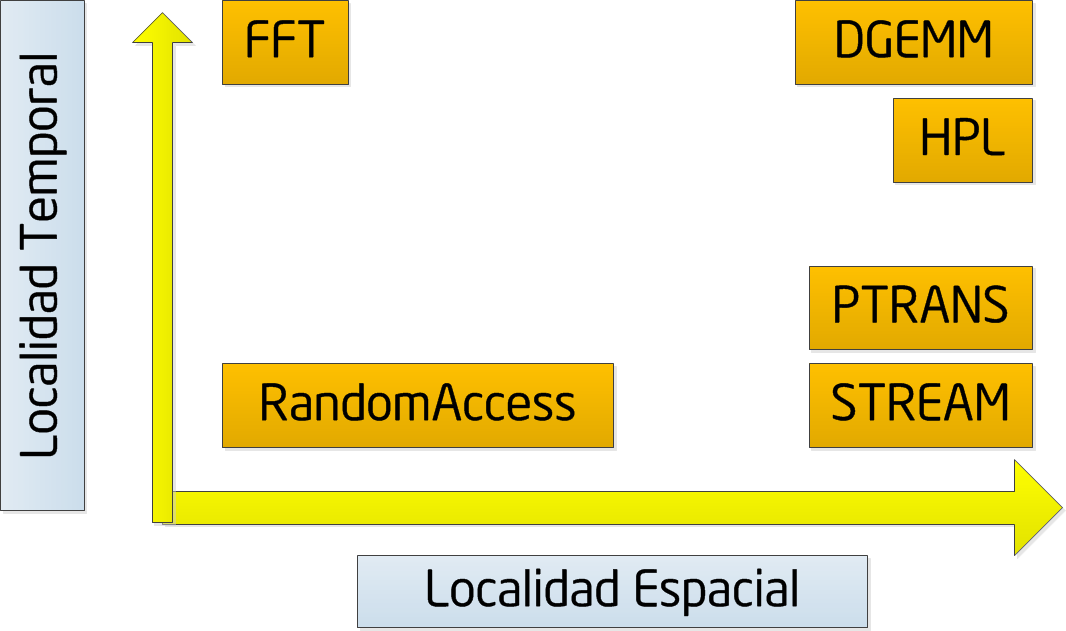
\includegraphics[width=10cm]{locality.png}
\caption{Localidad temporal versus espacial en resultados de HPCC}
\label{fig:locality}
\end{center}
\end{figure}

Para una mejor comparación de resultados de HPCC se utilizan diagramas de tipo radar denominados {\it kiviats}, un ejemplo se muestra en la Figura \ref{fig:kiviat}.
Los resultados están normalizados hacia uno de los sistemas, en este ejemplo se puede identificar mejor rendimiento en FLOPs por poseer mejores DGEMM y HPL en comparación.

\begin{figure}[H]
\begin{center}
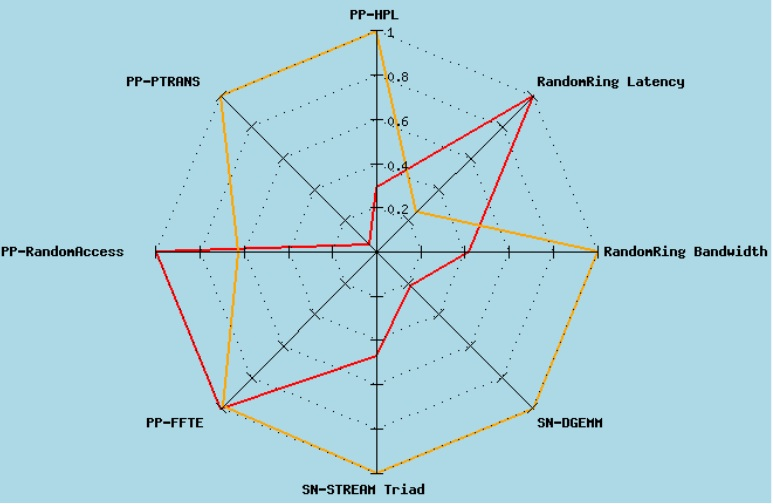
\includegraphics[width=12cm]{kiviat.png}
\caption{Diagrama Kiviat [Top500]}
\label{fig:kiviat}
\end{center}
\end{figure}

Un ejemplo de la salida que se muestra durante la ejecución se muestra a continuación.

{\scriptsize

\begin{verbatim}
This is the DARPA/DOE HPC Challenge Benchmark version 1.2.0 October 2003
Produced by Jack Dongarra and Piotr Luszczek
Innovative Computing Laboratory
University of Tennessee Knoxville and Oak Ridge National Laboratory

Begin of Summary section.
\end{verbatim}

\begin{minipage}[b]{0.5\linewidth}
\begin{verbatim}
VersionMajor=1
VersionMinor=2
LANG=C
Success=1
CommWorldProcs=3
MPI_Wtick=1.000000e-06
HPL_Tflops=0.0674008
HPL_time=26.3165
HPL_eps=1.11022e-16
HPL_N=13856
HPL_NB=64
HPL_nprow=1
HPL_npcol=3
HPL_depth=2
HPL_nbdiv=2
HPL_nbmin=8
HPL_cpfact=C
HPL_crfact=R
HPL_ctop=1
HPL_order=R
dweps=1.110223e-16
sweps=5.960464e-08
HPLMaxProcs=3
HPLMinProcs=3
DGEMM_N=4618
StarDGEMM_Gflops=68.9053
SingleDGEMM_Gflops=70.2692
PTRANS_GBs=0.794254
PTRANS_time=0.479293
PTRANS_residual=0
PTRANS_n=6928
PTRANS_nb=64
PTRANS_nprow=1
PTRANS_npcol=3
MPIRandomAccess_N=134217728
MPIRandomAccess_time=30.4475
MPIRandomAccess_Check=14.0705
MPIRandomAccess_Errors=0
\end{verbatim}
\end{minipage}
\hspace{0.1cm}
\begin{minipage}[b]{0.5\linewidth}
\begin{verbatim}
MPIRandomAccess_ErrorsFraction=0
MPIRandomAccess_ExeUpdates=536870912
MPIRandomAccess_GUPs=0.0176327
MPIRandomAccess_TimeBound=-1
MPIRandomAccess_Algorithm=0
RandomAccess_N=33554432
StarRandomAccess_GUPs=0.0186362
SingleRandomAccess_GUPs=0.0184568
STREAM_VectorSize=21332081
STREAM_Threads=8
StarSTREAM_Copy=4.34705
StarSTREAM_Scale=3.24366
StarSTREAM_Add=3.41196
StarSTREAM_Triad=3.46198
SingleSTREAM_Copy=4.53628
SingleSTREAM_Scale=3.38984
SingleSTREAM_Add=3.59073
SingleSTREAM_Triad=3.65083
FFT_N=8388608
StarFFT_Gflops=2.17339
SingleFFT_Gflops=2.26806
MPIFFT_N=8388608
MPIFFT_Gflops=1.7043
MPIFFT_maxErr=1.77722e-15
MPIFFT_Procs=2
MaxPingPongLatency_usec=5.37932
RandomRingLatency_usec=5.70686
MinPingPongBandwidth_GBytes=0.675574
NaturalRingBandwidth_GBytes=0.531278
RandomRingBandwidth_GBytes=0.529161
MinPingPongLatency_usec=5.24521
AvgPingPongLatency_usec=5.30978
MaxPingPongBandwidth_GBytes=0.682139
AvgPingPongBandwidth_GBytes=0.678212
NaturalRingLatency_usec=5.79357
FFTEnblk=16
FFTEnp=8
FFTEl2size=1048576
\end{verbatim}
\end{minipage}

\begin{verbatim}
End of Summary section.
End of HPC Challenge tests.
\end{verbatim}
}

\subsection{Utilización de las Herramientas}

Se recomienda un proceso de aplicación gradual empezando por herramientas generales de alto nivel que analizan la aplicación como un todo; terminando con herramientas de bajo nivel que proveen
detalles complejos de granularidad más fina en partes específicas del código. Esto permite ir analizando el rendimiento sin tener que enfrentar la dificultad de un análisis complejo y
extensivo desde un principio. Una lista de las herramientas más conocidas se muestra en la Tabla \ref{table:tooling}.

\begin{table}[H]
\caption{Aplicación Gradual de Herramientas}
\begin{tabular}{|l|l|} \hline
{\bf Característica} & {\bf Herramientas} \\ \hline
Capacidad del sistema & Benchmark HPCC \\ \hline
Medición de ejecución & {\tt time}, {\tt gettimeofday()}, {\tt MPI\_WTIME()} \\ \hline
Perfil de ejecución & profilers: {\tt gprof}, {\tt perf} \\ \hline
Comportamiento de la aplicación & profilers: {\tt gprof, perf} \\ \hline
Comportamiento de librerías & profilers: valgrind, MPI vampir. \\ \hline
Comportamiento del sistema & profilers: oprofile, perf \\ \hline
Vectorización & compilador: gcc \\ \hline
Contadores en {\it hardware} & oprofile, PAPI, perf \\ \hline
\end{tabular}
\label{table:tooling}
\end{table}

A grandes rasgos el procedimiento es el siguiente:

\begin{enumerate}

\item Se establece una línea de comparación al ejecutar una prueba de rendimiento del sistema, {\it HPCC} brinda un conjunto de métricas muy completo. 

\item Se utilizan herramientas para medir el tiempo de ejecución de la aplicación sobre diferentes escenarios. {\tt time} permite una ejecución directa sin modificación de código,
{\tt gettimeofday()} requiere modificación de código pero puede ser utilizados con mayor libertad dentro de la aplicación.  
En el caso de estar utilizando la librería MPI, {\tt MPI\_WTime()} y la herramienta VAMPIR\footnote{\href{http://www.vampir.eu}{http://www.vampir.eu}} proveen soporte específico para análisis
de rendimiento.

\item Se dimensiona el comportamiento de la aplicación mediante un perfil de ejecución y un análisis de cuello de botella utilizando {\tt gprof}. 

\item Se analiza el comportamiento del sistema ejecutando la aplicación mediante {\tt oprofile} \footnote{\href{http://oprofile.sourceforge.net}{http://oprofile.sourceforge.net}} o
{\tt perf} \footnote{\href{https://perf.wiki.kernel.org}{https://perf.wiki.kernel.org}}. 

\item Se revisa el reporte del compilador para comprobar que se estén vectorizando los ciclos de cálculo más intensivos.

\item Se analiza el comportamiento de las unidades de cómputo utilizando soporte de {\it hardware} mediante herramientas como {\tt perf}, {\tt oprofile} y {\it Performance Application Programming Interface} (PAPI) \footnote{\href{http://icl.cs.utk.edu/papi}{http://icl.cs.utk.edu/papi}}.

\end{enumerate}

\subsection{Tiempo de Ejecución}

Esta sección revisa como medir el tiempo de ejecución global de una aplicación, incluyendo ejemplos.

\subsubsection{Tiempo de ejecución global}

Para medir el tiempo de ejecución de un comando en consola se utiliza {\tt time(1)}. Aunque rudimentaria, esta simple herramienta no necesita de instrumentación de código y
se encuentra disponible en cualquier distribución {\it GNU/Linux}.
El intérprete de comandos tiene su propia versión embebida, sin embargo el del sistema brinda información del uso de otros recursos del sistema, usualmente localizado en {\tt /usr/bin/time}.
Un ejemplo se demuestra en el listado \ref{lst:time1}.

\bigskip

\begin{lstlisting}[caption={Ejecución del Programa},label={lst:time1}]
$ /usr/bin/time -v ./program
1
        Command being timed: "./program"
        User time (seconds): 0.61
        System time (seconds): 0.00
        Percent of CPU this job got: 99%
        Elapsed (wall clock) time (h:mm:ss or m:ss): 0:00.62
        Average shared text size (kbytes): 0
        Average unshared data size (kbytes): 0
        Average stack size (kbytes): 0
        Average total size (kbytes): 0
        Maximum resident set size (kbytes): 4560
        Average resident set size (kbytes): 0
        Major (requiring I/O) page faults: 0
        Minor (reclaiming a frame) page faults: 668
        Voluntary context switches: 6
        Involuntary context switches: 2
        Swaps: 0
        File system inputs: 0
        File system outputs: 0
        Socket messages sent: 0
        Socket messages received: 0
        Signals delivered: 0
        Page size (bytes): 4096
        Exit status: 0
\end{lstlisting}

\subsubsection{Reloj del sistema}

La librería principal de sistema permite acceder a llamadas al sistema operativo para obtener datos precisos del paso del tiempo.
Las más utilizadas son {\tt gettimeofday(3)} y {\tt clock(3)}, aunque éste último se comporta de manera especial al utilizar multi-threading ya que suma el tiempo ejecutado en cada unidad de
cómputo.

\bigskip

El código en el listado \ref{lst:wtime} ejemplifica como obtener un número de segundos en una representación de punto flotante de doble precisión, permitiendo una granularidad de medición
adecuada.

\begin{lstlisting}[caption={Tiempo de Ejecución},label={lst:wtime}]
double wtime(void)
{
  double sec;
  struct timeval tv;
  
  gettimeofday(&tv, NULL);
  sec = tv.tv_sec + tv.tv_usec/1000000.0;
  return sec;
}
\end{lstlisting}

\subsection{Perfil de Ejecución Funcional}

Las herramientas de perfilado denominadas {\it profilers} extraen el perfil dinámico de una aplicación en tiempo de ejecución. 
Se instrumenta la aplicación con una opción específica que incluye información de uso de las diferentes partes del programa y los recursos del sistema como por ejemplo procesador y memoria.

\bigskip

La aplicación debe ejecutarse con un conjunto de datos prefijado. El conjunto de datos debe ser representativo y debe también ejercitar la aplicación por
una cantidad de tiempo suficiente como para intensificar el uso de los recursos. Los datos del perfil de una ejecución son luego obtenidos en la
forma de un archivo de datos, luego se procede a procesar los datos acumulados con un analizador respectivo.

\bigskip

Provee un perfil plano que consiste en una simple lista de las funciones ejecutadas ordenadas por la cantidad acumulada de tiempo utilizado.
También provee el gráfico de llamadas anidadas, que muestra el tiempo utilizado por cada función en llamadas sucesivas. Las funciones recursivas
son manejadas de manera especial ya que imposibilitan el armado de relaciones de dependencias.

\subsubsection{Ejemplo: {\tt gprof}}

El perfil de ejecución de {\tt gprof} muestra el tiempo individual y el tiempo acumulado en segundos de cada línea de código de la aplicación. Los binarios deben ser compilados con información extra de depuración, en el caso de {\tt gcc}, las opciones necesarias son {\tt -g -pg}. Si {\tt -g} no se encuentra presente entonces no se provee el reporte detallado por línea de ejecución. Esto permite identificar donde se está consumiendo tiempo durante la ejecución.
La herramienta también muestra un cuadro de las llamadas entre funciones realizadas por el programa.
Esto permite visualizar el esquema de dependencias durante la ejecución.

\bigskip

A continuación en el listado \ref{debug} se muestra como realizar la compilación incluyendo información de depuración específica, además de un caso concreto contra una aplicación simulando el juego de la vida \cite{conway}.

\begin{lstlisting}[caption={Compilación con Información de Depuración},label={debug}]
$ gcc -g -pg program.c -o program
$ ./program
$ gprof program
...
\end{lstlisting}

En el listado \ref{lst:gprof} se muestra la información de las funciones del programa ordenadas por mayor impacto en el tiempo de ejecución.

\begin{lstlisting}[caption={Perfil de Rendimiento},label={lst:gprof}]
Flat profile:
Each sample counts as 0.01 seconds.
% cumulative self self total
time seconds seconds calls us/call us/call name
37.50 0.15 0.15 48000 3.12 3.12 Life::neighbor_count(int, int)
...
\end{lstlisting}

En el listado \ref{lst:call} se muestra la información del gráfico de llamadas del programa.

\begin{lstlisting}[caption={Gráficos de Llamadas},label={lst:call}]
Call graph
granularity: each sample hit covers 4 byte(s) for 2.50% of 0.40 seconds
index % time    self  children    called     name
      0.02 0.15 12/12 main [2]
[1] 42.5 0.02 0.15 12 Life::update(void) [1]
      0.15 0.00 48000/48000 Life::neighbor_count(int, int) [4]
--
          0.00    0.17       1/1           _start [3]
[2]     42.5    0.00    0.17       1         main [2]
          0.02    0.15      12/12          Life::update(void) [1]
          0.00    0.00      12/12          Life::print(void) [13]
          0.00    0.00      12/12          to_continue(void) [14]
          0.00    0.00       1/1           instructions(void) [16]
          0.00    0.00       1/1           Life::initialize(void) [15]
--
\end{lstlisting}

\subsection{Perfil de Ejecución Asistido por {\it Hardware}}

Un {\it profiler} puede utilizar el {\it hardware} para analizar el uso de los recursos disponibles a nivel de núcleo del sistema operativo. 
Actúa de forma transparente a nivel global. Utiliza contadores de {\it hardware} del CPU y además interrupciones de un temporizador
cuando no logra detectar soporte específico en {\it hardware}. Aunque tiene un costo adicional inherente, la sobrecarga es mínima.

\bigskip

Para obtener un perfil de ejecución representativo, usualmente se recomienda detener toda aplicación o servicio no relevante en el sistema. 
La herramienta de por si no requiere acceder al código fuente de la aplicación, pero si esta disponible el código correspondiente se muestra anotado con contadores
si hay símbolos de depuración en el binario.

\bigskip

Los registros de {\it hardware} implementando contadores más utilizados son los siguientes:

\begin{enumerate}
\item Cantidad total de ciclos de procesador
\item Cantidad total de instrucciones ejecutadas
\item Cantidad de ciclos detenidos por espera de acceso a memoria
\item Cantidad de instrucciones de punto flotante
\item Cantidad de fallos de cache de nivel uno (L1)
\item Cantidad de instrucciones de carga y descarga
\end{enumerate}

En núcleos {\it Linux} más nuevos que la versión 2.6, en lugar de {\tt oprofile} se recomienda utilizar {\tt perf}. Al estar implementados a nivel de núcleo, éstos evitan las llamadas al sistema y tienen una sobrecarga de un orden de magnitud menor que los {\it profilers} a nivel de aplicación. Las herramientas propietarias suelen tener acceso a contadores más específicos e
incluso programables para funciones determinadas de medición.

\subsubsection{Ejemplo: {\tt perf}}

A continuación en el listado \ref{lst:perfstat} se demuestra la información provista por {\tt perf} en sus diferentes modos de ejecución: estadísticas de contadores, perfil de sistema y
por último perfil de aplicación.

\begin{lstlisting}[caption={Estadísticas de Contadores},label={lst:perfstat}]
$ perf stat -B program
Performance counter stats for 'program':
           5,099 cache-misses  0.005 M/sec (scaled from 66.58%)
         235,384 cache-references 0.246 M/sec (scaled from 66.56%)
       9,281,660 branch-misses 3.858 %     (scaled from 33.50%)
     240,609,766 branches 251.559 M/sec (scaled from 33.66%)
   1,403,561,257 instructions  0.679 IPC   (scaled from 50.23%)
   2,066,201,729 cycles 2160.227 M/sec (scaled from 66.67%)
             217 page-faults 0.000 M/sec
               3 CPU-migrations 0.000 M/sec
              83 context-switches 0.000 M/sec
      956.474238 task-clock-msecs 0.999 CPUs
      0.957617512  seconds time elapsed
\end{lstlisting}

En el listado \ref{lst:record} se muestra la salida del perfil de rendimiento. Notar que se incluye incluso la información del comportamiento del núcleo del sistema.

\begin{lstlisting}[caption={Perfil de Rendimiento},label={lst:record}]
$ perf record ./mm
$ perf report
# Events: 1K cycles
# Overhead Command Shared Object Symbol
28.15% main mm [.] 0xd10b45
4.45% swapper  [kernel.kallsyms] [k] mwait_idle_with_hints
4.26% swapper  [kernel.kallsyms] [k] read_hpet
...
\end{lstlisting}

En el listado \ref{lst:annotated} se muestra la salida del perfil de código anotado con las instrucciones del ensamblador respectivas.

\begin{lstlisting}[caption={Código Anotado},label={lst:annotated}]
 Percent |   Source code & Disassembly of program
         :   Disassembly of section .text:
         :   08048484 <main>:
         :   #include <string.h>
         :   #include <unistd.h>
         :   #include <sys/time.h>
         :
         :   int main(int argc, char **argv)
         :   {
0.00:    8048484:       55                      push   %ebp
0.00:    8048485:       89 e5                   mov    %esp,%ebp
...
0.00:    8048530:       eb 0b                   jmp 804853d <main+0xb9>
         :                           count++;
14.22:    8048532:       8b 44 24 2c             mov    0x2c(%esp),%eax
0.00:    8048536:       83 c0 01                add    $0x1,%eax
14.78:    8048539:       89 44 24 2c             mov    %eax,0x2c(%esp)
         :           memcpy(&tv_end, &tv_now, sizeof(tv_now));
         :           tv_end.tv_sec += strtol(argv[1], NULL, 10);
         :           while (tv_now.tv_sec < tv_end.tv_sec ||
         :                  tv_now.tv_usec < tv_end.tv_usec) {
         :                   count = 0;
         :                   while (count < 100000000UL)
14.78:    804853d:       8b 44 24 2c             mov    0x2c(%esp),%eax
56.23:    8048541:       3d ff e0 f5 05          cmp    $0x5f5e0ff,%eax
0.00:    8048546:       76 ea                   jbe 8048532 <main+0xae>
...
\end{lstlisting}

Este punto de análisis requiere conocimiento avanzado de como funciona el CPU utilizado, su acceso a memoria y los costos de las diferentes instrucciones soportadas. 
Una fuente de consulta debe incluir conceptos generales de arquitectura de procesadores \cite{hennessy} e información de los fabricantes \cite{intel-optimization}.

\subsection{Reporte de Vectorización}

Una herramienta de bajo nivel para analizar rendimiento es el mismo compilador que debería estar vectorizando los ciclos de cómputo intensivo. Esto es muy
útil para detectar si los cuellos de botella ya se encuentran optimizados o no.

\bigskip

Por ejemplo, GCC provee opciones específicas que deben ser provistas para mostrar el reporte.
En el listado \ref{lst:vector} se muestra la información incluída.

\begin{lstlisting}[caption={Información de Vectorización},label={lst:vector}] 
$ gcc -c -O3 -ftree-vectorizer-verbose=1 ex.c
ex.c:7: note: LOOP VECTORIZED.
ex.c:3: note: vectorized 1 loops in function.
$ gcc -c -O3 -ftree-vectorizer-verbose=2 ex.c
ex.c:10: note: not vectorized: complicated access pattern.
ex.c:10: note: not vectorized: complicated access pattern.
ex.c:7: note: LOOP VECTORIZED.
ex.c:3: note: vectorized 1 loops in function.
$ gcc -c -O3 -fdump-tree-vect-details ex.c
...
\end{lstlisting}

En el caso de existir código recursivo, podemos comprobar que no suele estar soportado por los compiladores actuales.
La información de vectorización sobre un código que posee recursividad se muestra en el listado \ref{lst:queen}

\begin{lstlisting}[caption={Vectorización de Código Recursivo},label={lst:queen}]
$ gcc -Wall -Wextra -O3 -ftree-vectorizer-verbose=4 -g queen.c
queen.c:22: note: vectorized 0 loops in function.
queen.c:35: note: vectorized 0 loops in function.
\end{lstlisting}

\chapter{Descripción del Problema} \label{Descripcion del Problema}

Este capítulo introduce el problema a resolver.

\section{Análisis de Rendimiento}

Este trabajo trata entonces de simplificar la tarea de análisis de rendimiento. 

\bigskip

El problema concreto sobre el que se trabaja es brindar automatización para ahorrar esfuerzo y minimizar el nivel de conocimiento requerido durante el desarrollo de aplicaciones de cómputo de
altas prestaciones.

\subsection{Problemas Usuales}

\subsubsection{Interacción Humana}

La interacción humana siempre es fuente de errores involuntarios, además de malgastar el tiempo de un investigador o desarrollador en tareas factibles de ser automatizadas. Usualmente una persona es requerida para ejecutar los programas, tabular los resultados y generar gráficos para su resumen.

\bigskip

El análisis de rendimiento requiere de una disciplina absoluta. Una de las tareas más demandantes de tiempo es la ejecución de un programa bajo distintas configuraciones para entender su comportamiento.

\subsubsection{Manejo de Herramientas}

El aprendizaje del correcto uso y aplicación de las herramientas demanda valioso tiempo.
Sin embargo las herramientas adecuadas permiten extraer información de rendimiento de mayor granularidad y calidad de la información, posibilitando tomar una mejor decisión a la hora de focalizar los esfuerzos de optimización.

\bigskip

El análisis requiere el correcto uso de matemática estadística para promediar resultados, descartar ejecuciones problemáticas y establecer límites en las mejoras. Es frecuente la utilización de una hoja de cálculo para centralizar los cálculos una vez tabulados los tiempos de ejecución y demás métricas de rendimiento.

\subsubsection{Recopilación de Datos y Representación de Resultados}

El análisis requiere la recopilación de datos relevantes al rendimiento sobre el comportamiento del programa y el sistema ejecutando el mismo. Cuáles son estas métricas, cómo obtenerlas y cómo representarlas para el análisis es una tarea no trivial que requiere tiempo y experiencia en el tema.

\subsubsection{Optimización Temprana}

La optimización temprana sin tener en cuenta datos cuantitativos puede implicar que un esfuerzo importante no tenga impacto alguno en el resultado global del tiempo de ejecución de un programa.

\subsubsection{Implementación Teórica de Algoritmos}

La implementación directa de un algoritmo matemático puede garantizar su correctitud pero no su eficiencia durante su ejecución. La reutilización de librerías de dominio público ofrecidas por
los fabricantes es siempre preferida ya que garantizan eficiencia con un mínimo esfuerzo de aprender como utilizarlas correctamente.

\subsection{Métodos de Optimización}

Los métodos usuales de optimización de un programa que ya utiliza un algoritmo adecuado son usualmente los siguientes:

\begin{description}
\item[Código:] se analiza el código fuente para mejorar la predicción de saltos, realizar {\it inlining} de rutinas muy utilizadas, alinear código y realizar {\it unrolling} de ciclos para posibilitar vectorización.
\item[Ejecución:] se analiza el código a nivel de ensamblador para comprobar el uso de instrucciones livianas o vectoriales, y además tratando de reducir el uso de registros.
\item[Memoria:] se analiza las estructuras de datos para incrementar la tasa de transferencia a memoria, minimizar fallas de cache, alinear datos y mejorar la localidad del acceso a los mismos.
\item[Precarga:] se analiza el uso de instrucciones de {\it hardware} para precargar datos en cache cuando los algoritmos predictivos no son suficientes.
\item[Punto Flotante:] se considera el relajamiento de las reglas de redondeo y representación según los estándares, intercambiando un mayor error acumulado por mejor velocidad de procesamiento
\end{description}

\section{Infrastructura de Soporte}

Los problemas usuales durante el análisis de rendimiento listados anteriormente reflejan la necesidad de utilizar soporte automátíco para la ejecución de pruebas de rendimiento, la recopilación de métricas relevantes y la generación de un reporte con gráficos comparativos e información de contexto. Los siguientes requerimientos son los necesarios para una infrastructura de análisis de rendimiento.

\subsection{Reusabilidad}

La infastructura debe ser aplicable a un gran rango de programas, no requiriendo su modificación.
Su instalación solo debe depender de la existencia previa de las mismas herramientas que un usuario podría ejecutar para obtener información relacionada al rendimiento de un programa. La infrastructura debe ser eficiente, no debe requerir ejecutar pruebas largas y tediosas cuando la información puede ser reusada.

\subsection{Configurabilidad}

La aplicación de las herramientas debe ser configurable en su totalidad mediante un archivo de configuración.
Los parámetros a configurar deberían incluir entre otros: la forma de compilar y ejecutar un programa, el rango de valores de entrada, el número de repeticiones de las diferentes ejecuciones del programa.

\subsection{Portabilidad}

La infrastructura debe ser implementada con un lenguaje portable, de ser posible basado en código abierto de forma que pueda ser revisada fácilmente por los usuarios para incluir nuevas fuentes de información o cambiar la forma en que las herramientas base son utilizadas.

\subsection{Extensibilidad}

La infrastructura debe poseer un diseño de fácil extensión, la incorporación de nuevas herramientas, gráficos o secciones dentro de un reporte debe ser una tarea trivial asumiendo que ya se conoce la forma manual de obtener la información requerida para ello.

\subsection{Simplicidad}

La infrastructura debe reutilizar las mismas herramientas disponibles en el sistema, de tal forma el usuario puede continuar el análisis de forma directa.
También debe generar archivos de soporte con la información pura de los comandos ejecutados y su salida sin depurar.
Debe ser posible completar un reporte entre un día de trabajo y otro sin la interacción con un usuario.

\chapter{Propuesta de Solución} \label{Propuesta de Solucion}

Este capítulo muestra la propuesta de solución, incluyendo el diseño de la misma a diferentes niveles.

\section{Procedimiento}

La Figura \ref{fig:procedure} muestra a grandes rasgos las etapas del proceso a automatizar.

\begin{figure}[H]
\label{fig:procedure}
\centering
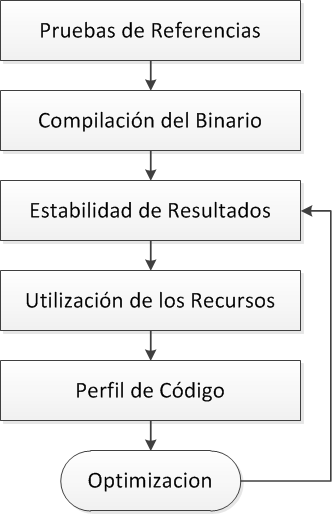
\includegraphics[width=5cm]{procedure.png}
\caption{Procedimiento de Análisis}
\end{figure}

Primero se establece una línea base de rendimiento del sistema utilizando pruebas de rendimiento conocidas.
Luego se procede a trabajar en etapas iterativas asegurando en cada paso la estabilidad de los resultados, revisando la utilización de recursos y utilizando un perfil de ejecución para encontrar un punto de enfoque. Luego de optimizar y comprobar la mejora, se vuelve a repetir el ciclo.

\section{Paso a Paso}

A continuación se muestran los pasos a realizar, junto con preguntas que guían el análisis de rendimiento de una aplicación.
La infrastructura solo implementa los pasos específicos de ejecución de herramientas para la recolección de información.

\subsection{Pruebas de Referencia}

\begin{enumerate}
\item Ejecutar pruebas de rendimiento sobre el sistema a utilizar para poder entender sus capacidades máximas en contraste con las teóricas.

\begin{lstlisting}[caption={Instalación de HPCC},label={lst:hpcc}]
$ sudo apt-get install hpcc
$ mpirun -n `grep -c proc /proc/cpuinfo` ./hpcc
$ cat hpccoutf.txt
\end{lstlisting}

\begin{enumerate}
\item ¿Los resultados reflejan las capacidades esperadas del sistema?
\item ¿Los FLOPS se aproximan al rendimiento de un sistema similar?
\item ¿El rendimiento es $ CORES \times CLOCK \times FLOPS/CYCLE $ ?
\item ¿La latencia y ancho de banda de la memoria es la esperada?
\end{enumerate}

\item Comprobar variación de resultados para conocer la estabilidad de los mismos. La desviación estándar debe ser menor a 3 sigmas. 
\item Establecer cual es el promedio geométrico a usar como referencia para comparaciones futuras.

\begin{lstlisting}[caption={Estabilidad de Resultados},label={lst:time}]
$ for i in `seq 1 32`; do /usr/bin/time -v ./program >> time.csv; done
\end{lstlisting}

\begin{enumerate}
\item ¿Son los resultados estables?
\item ¿La desviación estándar es menor que 3?
\item ¿Cuál es el promedio geométrico para comparaciones futuras?
\item ¿Es necesario incrementar el problema para mejorar la desviación?
\item ¿Es posible reducir el tiempo sin afectar la desviación?
\end{enumerate}

\item Escalar el problema para dimensionar la cantidad de trabajo según el tamaño del problema.

\begin{lstlisting}[caption={Escalamiento de Problema},label={lst:size}]
$ for size in `seq 1024 1024 10240`; do /usr/bin/time -v ./program $size >> size.log; done
\end{lstlisting}

\begin{enumerate}
\item ¿Cuál es la relación entre el tiempo de las diferentes ejecuciones?
\item ¿Es la incremento del tiempo de ejecución lineal o constante?
\end{enumerate}

\item Escalar cómputo para luego calcular límite de mejoras con {\it Amdalah} y {\it Gustafson}.

\begin{lstlisting}[caption={Escalamiento de Cómputo},label={lst:proc}]
$ for threads in `grep -c proc /proc/cpuinfo | xargs seq 1`; do OMP_NUM_THREADS=$threads ./program >> threads.log; done
\end{lstlisting}

\begin{enumerate}
\item ¿Cuál es la relación entre el tiempo de las diferentes ejecuciones?
\item ¿Es la relación lineal o constante?
\item ¿Qué porcentaje de la aplicación se estima paralelo?
\item ¿Cual es la mejora máxima posible?
\end{enumerate}

\item Generar el perfil de llamadas a funciones dentro de la aplicación para revisar el diseño de la misma y los posibles cuellos de botella a resolver.

\begin{lstlisting}[caption={Generación de Perfil de Rendimiento},label={lst:gprofall}]
$ gcc -g -pg program.c -o program
$ ./program
...
$ gprof --flat-profile --graph --annotated-source app
...
\end{lstlisting}

\begin{enumerate}
\item ¿Cómo está diseñada la aplicación?
\item ¿Que dependencias en librerías externas tiene?
\item ¿Implementa algún núcleo de cómputo conocido encuadrado dentro de librerías optimizadas como BLAS?
\item ¿En que archivos, funciones y líneas se concentra la mayor cantidad de tiempo de cómputo?
\end{enumerate}

\item Utilizar el profiler a nivel de sistema

\begin{lstlisting}[caption={Generación de Perfil de Sistema},label={lst:profall}]
$ prof stat ./program
$ prof record ./program
$ prof report
\end{lstlisting}

\begin{enumerate}
\item ¿Cómo se comporta el sistema durante la ejecución de la aplicación?
\item ¿Son las métricas de contadores de {\it hardware} las esperadas?
\item ¿Es la aplicación la gran concentradora de los recursos disponibles?
\item ¿Qué instrucciones de {\it hardware} son las mayormente utilizadas?
\end{enumerate}

\item Comprobar vectorizaciones

\begin{lstlisting}[caption={Información de Vectorización},label={lst:report}]
$ gcc -Wall -Wextra -O3 --report-loop
\end{lstlisting}

\begin{enumerate}
\item ¿Hay ciclos que no pueden ser automáticamente vectorizados?
\item ¿Pueden los ciclos no optimizados ser modificados?
\end{enumerate}

\end{enumerate}

\section{Infraestructura}

El procedimiento anterior se implementó como una infrastructura automática de generacion de reportes de rendimiento denominada 
{\tt hotspot} \footnote{El proyecto {\tt hotspot} está disponible en \href{https://github.com/moreandres/hotspot}{https://github.com/moreandres/hotspot}}.

\bigskip

La automatización se comporta del mismo modo que un usuario realizando un procedimiento sistemático de analisis de rendimiento.
Es decir que ejecuta utilidades del sistema como {\tt gcc}, {\tt make}, {\tt prof}, {\tt gprof}, {\tt pidstat} para obtener la información relevante.
\LaTeX se utiliza para la generación del reporte final.

\bigskip

Las limitaciones {\it a-priori} que posee la infrastructura son en materia de portabilidad y aplicación. Por el lado de la portabilidad, sólo se soportan sistemas {\it GNU/Linux recientes}, siendo necesarias el conjunto de utilidades de soporte especificadas anteriormente. Por el lado de la aplicación, sólo se soportan programan utilizando tecnología {\it OpenMP}.

\section{Teoría de Operación}

Esta sección detalla el funcionamiento de la infraestructura relacionando los componentes.

\subsection{Arquitectura}

A grandes rasgos el usuario utiliza la infrastructura para analizar un programa.
La infrastructura ejercita el programa múltiples veces hasta obtener la información necesaria para generar un reporte resumiendo los resultados.

\bigskip

La interacción con la infrastructura se detalla en la Figura \ref{fig:hotspot-seq} a continuación.

\begin{figure}[H]
\begin{center}
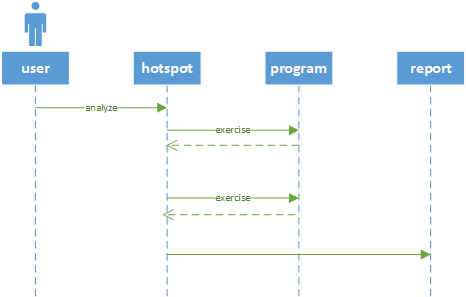
\includegraphics[width=\textwidth]{hotspot-seq.png}
\caption{Diagrama de Secuencia}
\label{fig:hotspot-seq}
\end{center}
\end{figure}

\subsection{Funcionamiento Interno}

Se utiliza un directorio escondido dentro de la carpeta que contiene la aplicación y se guardan en sub-directorios por fecha y hora las diferentes ejecuciones. 
Esta información puede ser usada para una comparación histórica de resultados.

\bigskip

Inicialmente se ejecuta la aplicación múltiples veces para validar que los resultados poseen una desviación saludable. Se resume esta información con un histograma y se hace una aproximación
a una distribución de resultados normales como comparación. Se toma como referencia la media geométrica de los resultados. La primer ejecución se descarta.

\bigskip

Se ejercita la aplicación dentro del rango de tamaño del problema especificado, por cada punto en el rango se ejecuta múltiples veces para luego tomar un promedio. Se grafican los resultados
en un gráfico de escalamiento donde se sobrepone una curva ideal suponiendo que un problema del doble de tamaño va a necesitar el doble de tiempo de cómputo.

\bigskip

Se detecta cuantas unidades de procesamiento hay en el sistema y se realizan pruebas utilizando más unidades incrementalmente. Se utiliza una y luego se itera hasta utilizar todas,
se ejecuta múltiples veces la aplicación y se promedia el resultado. También se sobrepone una curva ideal suponiendo escalamiento ideal como en el caso anterior.

\bigskip

Utilizando la información anterior, se calcula el porcentaje de ejecución en serie y en paralelo. Con esta información se calculan también los limites según leyes de {\it Amdalah} y
{\it Gustafson} para los procesadores disponibles y para un número grande como para visualizar el caso de poseer infinitas unidades de cómputo.

\bigskip

Se recompila la aplicación con información extra de depuración y se obtiene información del perfil de ejecución. Se detallan las funciones, las líneas de código y el
{\it assembler} implementado por las mismas.

\section{Diseño de Alto Nivel}

El diseño de la infrastructura refleja la interacción manual con el sistema. 
Se depende de la presencia de herramientas de línea de comando, del programa a analizar en particular, y de \LaTeX.
Estos componentes se detallan en la Figura \ref{fig:hotspot-hld}.

\begin{figure}[H]
\begin{center}
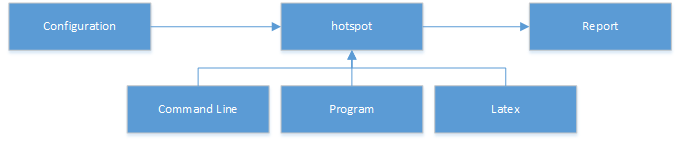
\includegraphics[width=\textwidth]{hotspot-hld.png}
\caption{Diseño de Alto Nivel}
\label{fig:hotspot-hld}
\end{center}
\end{figure}

\begin{enumerate}
\item{\bf Configuración}: el componente lee información de configuración y la deja disponible para los demás componentes.
\item{\bf Reporte}: el componente guarda valores de variables que luego utiliza para generar el reporte final. 
\item{\bf Infrastructura}: este componente utiliza información de configuración para generar ejercitar el programa y generar un reporte con los resultados.
\end{enumerate}

La siguiente sección revisa más en detalle como la infrastructura está compuesta internamente.

\section{Diseño de Bajo Nivel}

La infrastructura se implementa mediante una jerarquía de clases bastante simple, siendo fácil de extender de ser necesario.
Las diferentes clases disponibles se muestran en la Figura \ref{fig:hotspot-lld}.

\begin{figure}[H]
\begin{center}
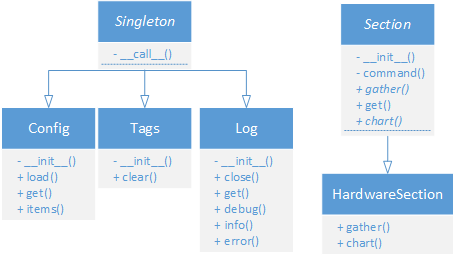
\includegraphics[width=\textwidth]{hotspot-lld.png}
\caption{Diseño de Bajo Nivel}
\label{fig:hotspot-lld}
\end{center}
\end{figure}

Aunque solo se incluye {\it HardwareSection} como ejemplo, existe un objeto sección por cada sección dentro del reporte.

A continuación se listan la totalidad de las clases junto con una descripción de las mismas.

\begin{enumerate}
\item {\it Singleton}: Patrón de Instancia Única. Es utilizado por otras clases para garantizar que solo existe una instancia única.
\item {\it Tags}: Almacenamiento de Palabras Clave. Es utilizado para guardar palabras clave que son utilizadas para generar el reporte.
\item {\it Log}: Generador de Mensajes. Es utilizado para estructurar los mensajes durante la ejecución.
\item {\it Config}: Administración de la Configuracion. Es utilizado para leer y consultar la configuración.
\item {\it Section}: Sección del Reporte. Es utilizado como base de otras secciones.
\item {\it HardwareSection}: Descripción del {\it Hardware}. Es utilizado para obtener información del {\it hardware} disponible.
\item {\it ProgramSection}: Detalles sobre el Programa. Es utilizado para obtener información del programa a analizar.
\item {\it SoftwareSection}: Descripción del {\it Software}, Es utilizado para obtener información del {\it software} disponible.
\item {\it SanitySection}: Chequeo Base. Es utilizado para comprobaciones básicas del programa.
\item {\it BenchmarkSection}: Pruebas de Rendimiento, Es utilizada para obtener información de rendimiento.
\item {\it WorkloadSection}: Caso de Prueba. Es utilizada para obtener información del caso de prueba.
\item {\it ScalingSection}: Escalamiento de Problema. Es utilizada para entender como escala el tamaño del problema.
\item {\it ThreadsSection}: Hilos. Es utilizada para entender como escalan las unidades de cómputo.
\item {\it OptimizationSection}: Optimización. Es utilizada para entender el efecto de los diferentes niveles de optimización del compilador.
\item {\it ProfileSection}: Sección sobre el Perfil de Rendimiento. Permite entender en que partes del programa se invierte el tiempo de ejecución.
\item {\it ResourcesSection}: Utilización de Recursos. Permite entender como se utilizan los recursos del sistema.
\item {\it AnnotatedSection}: Código Anotado. Incluye código ensamblador de los cuellos de botella. 
\item {\it VectorizationSection}: Vectorización de Ciclos. Es utilizado para entender cuales ciclos fueron vectorizados o no.
\item {\it CountersSection}, Información de Contadores de {\it Hardware}. Es utilizado para resumir la información de los contadores de {\it hardware}.
\item {\it ConfigSection}, Configuración. Es utilizado para revisar la configuración del análisis.
\end{enumerate}

\subsection{Implementación}

La implementación se desarrolló sobre una plataforma {\it GNU/Linux}, utilizando la distribución {\tt Ubuntu 14.04.1 LTS}.
El lenguaje utilizado {\tt Python 2.7.6}, publicado en {\it Python Software Foundation Package Index} como {\tt hotspot} versión 0.3.
El repositorio de código también se encuentra disponible \footnote{\href{https://github.com/moreandres/hotspot}{https://github.com/moreandres/hotspot}}.
La licencia del código fuente es GPLv2. Se reutilizan librerías como {\tt matplotlib.pyplot} \cite{matplotlib} y {\tt numpy} \cite{numpy} para gráficar los resultados obtenidos durante las pruebas de rendimiento.

\subsection{Archivos}

Una vez instalado el paquete en el sistema, cualquier modificación es posible ya que se utiliza un lenguaje interpretado. 
Como referencia rápida, la ubicación de los archivos suele ser: \\ {\tt /usr/local/lib/python2.7/dist-packages/hotspot-0.0.2-py2.7.egg}.

\begin{description}
\item[Lógica Principal]: La lógica que obtiene información para ser incluida en el reporte se puede encontrar en {\tt hotspot/hotspot.py}.
\item[Plantilla del Reporte]: La plantilla \LaTeX que contiene el formato del reporte se puede encontrar en {\tt config/hotspot.tex}.
\item[Configuración]: Un archivo de configuración de ejemplo puede encontrarse en {\tt config/hotspot.cfg}.
\end{description}

\subsection{Configuración}

El listado \ref{lst:hotspot-help} muestra la pantalla de ayuda de la infrastructura.
La herramienta de línea de comando toma como parámetro principal un archivo de configuración donde se describen las características del programa a analizar. 

\begin{lstlisting}[language=bash, caption={Ayuda de {\tt hotspot}}, label={lst:hotspot-help}]
$ hotspot --help
usage: hotspot [-h] [-v] [--config CONFIG] [--debug]

Generate performance report for OpenMP programs.

optional arguments:
  -h, --help            show this help message and exit
  -v, --version         show program's version number and exit
  --config CONFIG, -c CONFIG
                        path to configuration
  --debug, -d           enable verbose logging

Check https://github.com/moreandres/hotspot for details.
\end{lstlisting}

\bigskip

Entre las características necesarias se incluye la forma de compilar la aplicación, ya que para algunos pasos de análisis se necesita incorporar información extra de depuración. El archivo de configuración también permite la definición de tareas como configuración y ejecución del programa con parámetros específicos de tamaño o resolución del problema de entrada. Otro parámetro necesario es el rango de tamaños de problema a utilizar durante las ejecuciones, definidos como una secuencia de formato compatible con la herramienta {\it Unix} {\tt seq} \footnote{\href{http://man.cat-v.org/unix\_8th/1/seq}{http://man.cat-v.org/unix\_8th/1/seq}}.

\bigskip

El archivo de configuración requerido se muestra en el listado \ref{lst:hotspot-config}.

\begin{lstlisting}[language=bash, caption={Configuración de {\tt hotspot}}, label={lst:hotspot-config}]
# hotspot configuration file

[hotspot]
# python format method is used to pass parameters

# range is a seq-like definition for problem size
range=1024,2048,256

# cflags are the compiler flags to use when building
cflags=-O3 -Wall -Wextra

# build is the command used to build the program
build=CFLAGS='{0}' make

# clean is the cleanup command to execute
clean=make clean

# run is the program execution command
run=OMP_NUM_THREADS={0} N={1} ./{2}

# count is the number of runs used to check for workload stabilization
count=16
\end{lstlisting}

\section{Reporte Generado}

A continuación se explica el contenido de cada sección del reporte generado en particular.
En el Apéndice \ref{examples} se adjuntan ejemplos utilizando núcleos de cómputo conocidos.

\subsection{Consideraciones Generales}

Las consideraciones generales tenidas en cuenta en todas las secciones fueron las siguientes:

\begin{description}
\item[Formato portable similar a un artículo de investigación:] Esto resulta en un documento que cualquiera puede consultar, con un formato familiar.
\item[Hipervínculos a archivos con la información pura:] Esto permite que al identificar algun punto interesante, se pueda consultar la información tal como fue producida por la herramienta en cuestión.
\item[Explicación breve del objetivo de la sección y/o gráficos:] Esto permite entender rápidamente la información de cada sección.
\item[Inclusión de líneas de tendencía y comportamiento ideal en gráficos:] Esto permite una rápida comparación con el escenario ideal.
\item[Referencias a material de consulta:] Esto permite ahondar en detalles en caso de ser necesario.
\item[Utilización del inglés:] Esto permite compartir los resultados fácilmente entre grupos de trabajos distribuídos internacionalmente.
\end{description}

\subsection{Consideraciones Particulares}

\subsubsection{Resumen}

El resumen incluído en la primer página introduce el reporte junto con información sobre la infrastructura utilizada y la ubicación de la información de ejecución.

\subsubsection{Contenido}

Contiene un índice de secciones en formato reducido de dos columnas con hipervínculos, de modo de facilitar la búsqueda rápida de la información.

\subsubsection{Programa}

Se incluyen detalles sobre el programa bajo análisis. Esto permite recordar la versión del programa, la fecha y hora exacta del análisis, y los parámetros de entrada utilizados.

\subsubsection{Capacidad del Sistema}

Se incluyen detalles sobre la configuración de {\it hardware} y {\it software} del sistema.
Esto permite comparar los resultados contra sistemas similares, o validar que una distinta configuración impacta o no en la ejecución del programa.

\bigskip

Además se incluye información de referencia obtenida de la prueba de rendimiento {\it HPCC}. Esto permite rápidamente entender las capacidades del sistema en núcleos de cómputo conocidos.

\subsubsection{Carga de Trabajo}

Se incluye información sobre el caso de prueba ejecutado. Se detalla el tamaño del mismo en memoria y la composición de sus estructuras ya que esto impacta directamente sobre la utilización de la jerarquía de memoria del sistema.

\bigskip

Se incluye también un resumen estadístico de la estabilidad del caso de prueba luego de repetirlo varias veces.
Un histograma muestra la distribución de los resultados y el promedio geométrico resultante a ser utilizado como línea base.

\bigskip

También se incluye un gráfico demostrando los tiempos de ejecución del caso de prueba bajo diferentes niveles de optimización en el compilador.
Esto permite entender el grado de optimización que ya posee un programa en materia de vectorización.

\subsubsection{Escalabilidad}

Se incluyen gráficos resumiendo la escalabilidad del programa al aumento el tamaño del problema y también por separado la cantidad de unidades de cómputo. 
Esto permite entender el grado de optimización del programa.

\bigskip

Se estima la proporción paralelo/lineal del programa, y junto con ellas se calculan mejoras teóricas máximas bajo las leyes de {\it Amdalah} y {\it Gustafson}.
Este dato es importante para entender el tope de mejora posible.

\subsubsection{Perfil de Ejecución}

Se incluye información sobre las funciones y líneas de código más usadas del programa durante su ejecución. 
Esto nos focaliza explícitamente los futuros esfuerzos de optimización, ya que garantiza un alto impacto global.

\bigskip

Se incluyen gráficos sobre el uso de los recursos del sistema durante una ejecución del programa. Incluyendo utilización de CPU, memoria y lectura/escritura de disco.

\bigskip

Se listan también cuellos de botella, junto con el código de ensamblador respectivo. Esta valiosa información nos permite entender que tipo de instrucciones se están utilizando para llevar a cabo el trabajo más intenso del programa.

\subsubsection{Bajo Nivel}

Se incluye el reporte de vectorización emitido por el compilador. Nos permite comprobar si todos los ciclos dentro del código fuente están siendo vectorizados. 
En caso negativo, se muestra información relevante de la razón.

\bigskip

Se incluye además el reporte de contadores de {\it hardware} relacionados con el rendimiento de la unidad de procesamiento. 
Aunque requiere un entendimiento avanzado de la arquitectura del sistema \cite{hennessy}, muchos problemas pueden ser identificados con esta información.

\subsubsection{Referencias}

Se incluye una lista de publicaciones relacionadas, las cuales son referenciadas en las secciones anteriores.
Esto permite a los usuarios del reporte conocer más de los puntos relevantes de cada sección si así lo desean.

\chapter{Casos de Aplicación} \label{Casos de Aplicacion}

Este capítulo contiene casos de estudio mostrando los resultados de aplicar la infraestructura desarrollada a aplicaciones de cómputo de alto rendimiento conocidas.

\section{Sistema de Prueba}

La configuración del sistema obtenida es la correcta teniendo en cuenta que las pruebas fueron realizadas sobre {\it hardware} virtualizado. La identificación de la memoria, procesador,
placa madre y almacenamiento pueden ser utilizados para buscar información de rendimiento publicada oficialmente por cada fabricante.

\bigskip

La identificación del {\it software} disponible en el sistema permite ser más específicos al comparar los resultados obtenidos.

\bigskip

La información de línea base de rendimiento obtenida luego de ejecutar el conjunto de pruebas de rendimiento contenido dentro de HPCC nos permite correlacionar núcleos de computo
conocidos contra los dominantes en nuestro programa bajo análisis.

\section{Código de Prueba}

Esta sección incluye una revisión de los resultados específicos obtenidos al aplicar la infrastructura a códigos de prueba.

\subsection{Multiplicación de Matrices}

La multiplicación de matrices es una operación fundamental en diversos campos de aplicación científica como la resolución de ecuaciones lineales y la representación de grafos y espacios dimensionales. Por ello existe abundante material sobre el tema. Tomando como ejemplo una implementación utilizando OpenMP \footnote{\href{http://blog.speedgocomputing.com/2010/08/parallelizing-matrix-multiplication.html}{http://blog.speedgocomputing.com/2010/08/parallelizing-matrix-multiplication.html}.}. El código utilizado se muestra continuación en el listado \ref{lst:matrix}, la configuración del caso de prueba en el listado \ref{lst:cfg-matrix}.

\bigskip

\begin{lstlisting}[caption={Código de Multiplicación de Matrices},label={lst:matrix}]
#include <stdlib.h>
#include <stdio.h>

int main()
{
  int size = 1024;
  if (getenv("N"))
    size = atoi(getenv("N"));

  float *a = malloc(sizeof(float) * size * size);
  float *b = malloc(sizeof(float) * size * size);
  float *c = malloc(sizeof(float) * size * size);
  
  int i, j, k;

  for (i = 0; i < size; ++i) {
    for (j = 0; j < size; ++j) {
      a[i+j*size] = (float) (i + j);
      b[i+j*size] = (float) (i - j);
      c[i+j*size] = 0.0f;
    }
  }

#pragma omp parallel for shared(a,b,c) 
  for (i = 0; i < size; ++i) {
    for (j = 0; j < size; ++j) {
      for (k = 0; k < size; ++k) {
	c[i+j*size] += a[i+k*size] * b[k+j*size];
      }
    }
  }

  return 0;
}
\end{lstlisting}

\bigskip

\begin{lstlisting}[caption={Caso de Prueba de Multiplicación de Matrices},label={lst:cfg-matrix}]
# hotspot configuration file
[hotspot]
range=1024,2048,256
cflags=-O3 -Wall -Wextra
build=CFLAGS='{0}' make
clean=make clean
run=OMP_NUM_THREADS={0} N={1} ./{2}
count=8
\end{lstlisting}

\bigskip

El reporte de rendimiento nos demuestra lo siguiente:

\begin{enumerate}

\item El caso de prueba es muy estable, con una desviación estandar mucho menor a 1.

\smallskip

Esto implica que el tamaño de los datos de entrada son apropiados para realizar un análisis de rendimiento sin introducir datos aleatorios de ejecución.

\item Las optimizaciones que realiza el compilador demuestran un impacto importante en el tiempo de ejecución.

\smallskip

Esto implica que las optimizaciones automáticas realizadas por el compilador encuentran en el código oportunidades claras de optimización.

\item Los tiempos de ejecución al escalar el problema descubren un pico que posiblemente implique un error de implementación de algoritmo.

\item Los tiempos de ejecución al incrementar las unidades de cómputo revelan un problema ya que no muestra mejoras constantes.

\item Se estima un 75\% de paralelismo, con una mejora teórica máxima de 3.5 veces sin escalar el tamaño del problema si utilizamos el mismo algoritmo.

\smallskip

Los últimos tres items muestran que la implementación del código no está optimizada para los recursos de cómputo disponibles. 

En este caso es recomendable la revisión de publicaciones en el tema y la reutilización de librerías ya optimizadas.

\item El cuello de botella se localiza en el código que obtiene el valor parcial de un elemento de la matriz resultante.

\item No hay lecturas ni escrituras al disco, por lo que no se está rendimiento al utilizar memoria virtual.

\smallskip

Esto implica que el tamaño elegido de problema puede ser cálculado integramente utilizando la memoria principal.

\item El cuello de botella principal utiliza la instrucción {\tt add}, la cual no es vectorial.

\smallskip

Esto implica que el código no está siendo totalmente vectorizado, desaprovechando la capacidad de cómputo disponible.

\item Las vectorizaciones no son realizadas exitosamente por el compilador en ningún ciclo dentro del código.

\smallskip

Esto implica que los ciclos de cómputos no están siendo vectorizados, desaprovechando la capacidad de cómputo disponible.

\end{enumerate}

El reporte generado por la infrastructura puede consultarse en el apéndice \ref{example-matrix}.
Una comparación de rendimiento de diferentes algoritmos de multiplicación de matrices puede encontrarse en \cite{mm-tool}.

\subsection{Transmisión de Calor en 2 Dimensiones}

Otro problema interesante es la simulación de transferencia de calor en un plano bidimensional.
Se utiliza una grilla donde cada celda transfiere calor a sus vecinos en una serie finita de ciclos simulando el paso del tiempo \footnote{\href{http://www.rblasch.org/studies/cs580/pa5/\#Source+Code-N100AC}{http://www.rblasch.org/studies/cs580/pa5/\#Source+Code-N100AC}.}. El código utilizado es incluido a continuación en el listado \ref{lst:heat}, la configuración del caso de prueba en el listado \ref{lst:cfg-heat}.

\bigskip

\begin{lstlisting}[caption={Código de Transmisión de Calor en 2 Dimensiones},label={lst:heat}]
#include <stdio.h>
#include <stdlib.h>
#include <math.h>

#define CRESN   302		/* x, y resolution */
#define RESN    300
#define MAX_COLORS 8
#define MAX_HEAT  20.0

double solution[2][CRESN][CRESN], diff_constant;
int cur_gen, next_gen;

double sim_time, final = 10000.0, time_step = 0.1, diff = 10000.0;

void compute_one_iteration();
void setup();

int main()
{
  final = 1024;
  if (getenv("N"))
    final = atoi(getenv("N"));

  int temp;

  setup ();

  for (sim_time = 0; sim_time < final; sim_time += time_step)
    {
      compute_one_iteration (sim_time);
      temp = cur_gen;
      cur_gen = next_gen;
      next_gen = temp;
    }

  return 0;
}

void setup()
{
  int i, j;

#pragma omp parallel for shared(solution) private(i,j)
  for (i = 0; i < CRESN; i++)
    for (j = 0; j < CRESN; j++)
      solution[0][i][j] = solution[1][i][j] = 0.0;

  cur_gen = 0;
  next_gen = 1;
  diff_constant = diff * time_step / ((float) RESN * (float) RESN);
}

void compute_one_iteration()
{
  int i, j;
  /* set boundary values */
  for (i = 0; i < CRESN; i++)
    {
      if (i < 256 || i > 768)
	solution[cur_gen][i][0] = solution[cur_gen][i][1];
      else
	solution[cur_gen][i][0] = MAX_HEAT;
    }
  for (i = 0; i < CRESN; i++)
    {
      solution[cur_gen][i][CRESN - 1] = solution[cur_gen][i][CRESN - 2];
    }
  for (i = 0; i < CRESN; i++)
    {
      solution[cur_gen][0][i] = solution[cur_gen][1][i];
      solution[cur_gen][CRESN - 1][i] = solution[cur_gen][CRESN - 2][i];
    }
  /* corners ? */

#pragma omp parallel for shared(solution,cur_gen,next_gen,diff_constant) private(i,j)
  for (i = 1; i <= RESN; i++)
    for (j = 1; j <= RESN; j++)
      solution[next_gen][i][j] = solution[cur_gen][i][j] +
	(solution[cur_gen][i + 1][j] +
	 solution[cur_gen][i - 1][j] +
	 solution[cur_gen][i][j + 1] +
	 solution[cur_gen][i][j - 1] -
	 4.0 * solution[cur_gen][i][j]) * diff_constant;
}
\end{lstlisting}

\bigskip

\begin{lstlisting}[caption={Caso de Prueba de Distribución de Calor en 2 Dimensiones},label={lst:cfg-heat}]
[hotspot]
range=16384,32768,1024
cflags=-O3 -Wall -Wextra
build=CFLAGS='{0}' make
clean=make clean
run=OMP_NUM_THREADS={0} N={1} ./{2}
count=8
\end{lstlisting}

\bigskip

Algunas conclusiones que pueden obtenerse son:

\begin{enumerate}
\item El caso de prueba es estable.
\item Las optimizaciones del compilador tienen impacto acotado.
\item El tiempo de ejecución al incrementar el tamaño del problema no crece monotónicamente.
\item El tiempo de ejecución al sumar más unidades de cómputo no decrece sistemáticamente.
\item El paralelismo en el programa solo alcanza el 50\%, por lo tanto el límite máximo de mejora es de 2 veces.
\item Hay dos cuellos de botella con un 25\% y un 15\% del tiempo de ejecución.
\item El 35\% del tiempo de ejecución lo ocupa la instrucción {\tt mov}.
\item Los ciclos no están siendo vectorizados.
\end{enumerate}

El reporte generado por la infrastructura puede consultarse en el apéndice \ref{example-heat2d}.

\subsection{Conjunto de {\it Mandelbrot}}

Los conjuntos de {\it Mandelbrot} resultan de un cálculo de una secuencia de operaciones sobre números complejos que no tienden a infinito.
Si se supone que los componentes real y complejo corresponden a las coordenadas de un gráfico de dos dimensiones, las imágenes resultantes simulan figuras fractales \cite{mandel}.
El código utilizado se incluye a continuación en el listado \ref{lst:mandel}, la configuración utilizada para el caso de prueba en el listado \ref{lst:cfg-mandel}.

\bigskip

\begin{lstlisting}[caption={Código de Conjunto de Mandelbrot},label={lst:mandel}]
#include <math.h>
#include <stdio.h>
#include <stdlib.h>
#include <string.h>
#include <assert.h>

#define X_RESN 1024
#define Y_RESN 1024
#define X_MIN -2.0
#define X_MAX 2.0
#define Y_MIN -2.0
#define Y_MAX 2.0

typedef struct complextype
{
  float real, imag;
} Compl;

int main()
{
  int i, j, k;
  Compl z, c;
  float lensq, temp;
  int iters;
  int res[X_RESN][Y_RESN];

  iters = 1024;
  if (getenv("N"))
    iters = atoi(getenv("N"));

#pragma omp parallel for shared(res, iters) private(i, j, z, c, k, temp, lensq)
  for (i = 0; i < Y_RESN; i++)
    for (j = 0; j < X_RESN; j++)
      {
	z.real = z.imag = 0.0;
	c.real = X_MIN + j * (X_MAX - X_MIN) / X_RESN;
	c.imag = Y_MAX - i * (Y_MAX - Y_MIN) / Y_RESN;
	k = 0;

	do
	  {
	    temp = z.real * z.real - z.imag * z.imag + c.real;
	    z.imag = 2.0 * z.real * z.imag + c.imag;
	    z.real = temp;
	    lensq = z.real * z.real + z.imag * z.imag;
	    k++;
	  }
	while (lensq < 4.0 && k < iters);

	if (k >= iters)
	  res[i][j] = 0;
	else
	  res[i][j] = 1;

      }

  assert(res[0][0]);

  return 0;
}
\end{lstlisting}

\bigskip

\begin{lstlisting}[caption={Caso de Prueba de Conjunto de Mandelbrot},label={lst:cfg-mandel}]
[hotspot]
range=16384,32768,1024
cflags=-O3 -Wall -Wextra
build=CFLAGS='{0}' make
clean=make clean
run=OMP_NUM_THREADS={0} N={1} ./{2}
count=8
\end{lstlisting}

\bigskip

Algunas conclusiones que pueden obtenerse al ejecutar la infrastructura desarrollada sobre una implementación básica son:

\begin{enumerate}
\item La estructura utilizada para representar números complejos está alineada y no posee huecos.
\item El caso de prueba es muy estable.
\item La proporción del trabajo en paralelo es demasiado alta e incluso mejor que un caso ideal. Esto refleja un problema ya que es imposible.
\item Cerca del 50\% del tiempo se invierte en una única línea de código.
\item Algunos ciclos ya se encuentran optimizados, se identifica el uso de instrucciones vectoriales como {\tt movss, addss}.
\end{enumerate}

\bigskip

El reporte generado puede consultarse en el apéndice \ref{example-mandel}.

\chapter{Conclusiones y Trabajo Futuro} \label{Conclusiones y Trabajo Futuro}

Este capítulo concluye revisando los objetivos propuestos y posibles líneas de investigación como continuación.

\section{Conclusiones}

La optimización del rendimiento de una aplicación es algo no trivial.
Es preciso realizar un análisis disciplinado del comportamiento y del uso de los recursos antes de
empezar a optimizar. Las mejoras pueden ser no significativas si son realizadas en el lugar incorrecto.

\bigskip

Este trabajo soporta los primeros pasos de análisis de rendimiento para expertos del dominio de un problema científico utilizando computación de altas prestaciones. Se provee una metodología de uso de herramientas de soporte para principiantes, que puede ser utilizada como una lista de pasos resumidos para usuarios casuales, e incluso como referencia de consulta diaria para expertos.

\bigskip

Se resume también el estado del arte del análisis de rendimiento en aplicaciones de cómputo de altas prestaciones. Respecto a herramientas de soporte, se detallan diferentes opciones y se demuestra su aplicación en varios problemas simples aunque suficientemente interesantes para mostrar los beneficios de un análisis automático. 

\bigskip

Este estudio propone un proceso de análisis de rendimiento gradual e iterativo para cualquier investigador. 
Incluyendo soporte automático para la aplicación de las herramientas y la generación integrada de
reportes de rendimiento.

\bigskip

Se desarrolló como estaba planeado una infrastructura de soporte que permite a un desarrollador especialista en el dominio de un problema obtener rápidamente información cuantitativa del comportamiento de un programa {\it OpenMP}, incluyendo utilización del recurso y cuellos de botella para dirigir los esfuerzos de optimización.

\bigskip

La infrastructura fue construída sobre los comandos que un desarrollador utilizaría. Realizar cualquier modificación es entonces trivial para contemplar nuevas herramientas
o agregar nuevas secciones en los reportes generados como etapa final.

\section{Trabajo Futuro}

Las posibilidades de extensión de esta infrastructura son muchas, cada sección del reporte final puede incluir información más detallada o utilizar otras herramientas. En particular la sección de contadores de {\it hardware} solo contiene una lista de contadores generalizada para cualquier arquitectura; si se asume una arquitectura dada, se puede fácilmente proveer información más especifica y por lo tanto más útil.

\bigskip

La utilización de estas ideas en una aplicación del mundo real es materia pendiente, otra posibilidad es re-implementar desde cero alguna aplicación
científica en colaboración con algún grupo de investigación y realizar varios ciclos de optimización para validar su utilidad.

\bigskip

Otra posibilidad consiste en incorporar soporte para programas basados en la librería de comunicación MPI. Una vez que los programas son optimizados para ejecutarse eficientemente sobre un solo sistema, el siguiente paso consiste en utilizar varios sistemas en conjunto como se detalla en \cite{beowulf-parallel-workstation} \cite{tinetti}.

\bigskip

Por último, aunque la generación de un documento portable en formato PDF es simple y útil, se puede pensar como siguiente paso en utilizar una tecnología que permita la generación de reportes dinámicos que permitan a los expertos modificar la representación de la información. Por ejemplo, una implementación en HTML5 o en un formato compatible con planillas de cálculo utilizando tablas filtrables y gráficos configurables puede ser interesante y mejorar la calidad del análisis de rendimiento.

\bibliography{report}

\appendix

\chapter{Reporte de Ejemplo} \label{examples}

\section{Multiplicación de Matrices}  \label{example-matrix}
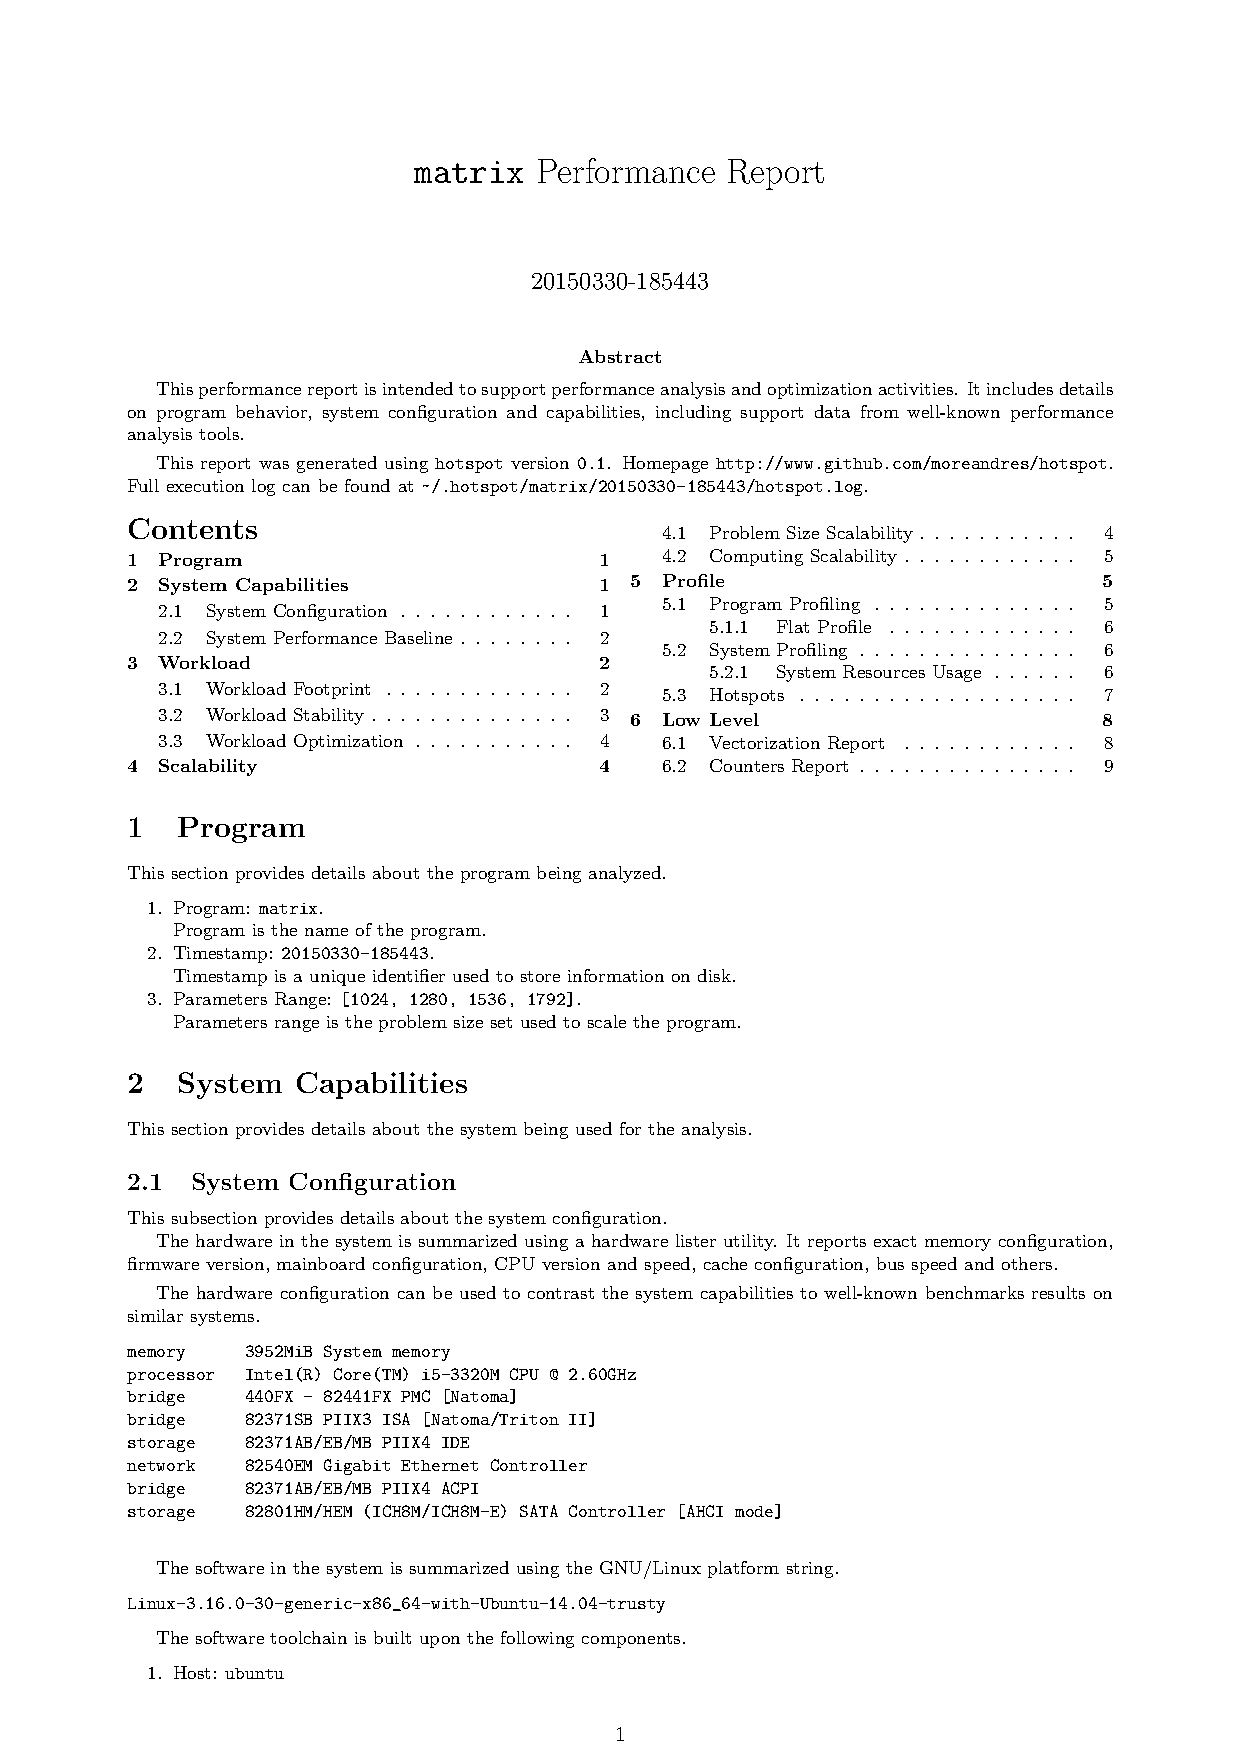
\includepdf[frame=true, pages=-, scale=0.75, pagecommand={}]{matrix.pdf}

\section{Propagación de Calor en 2 Dimensiones} \label{example-heat2d}
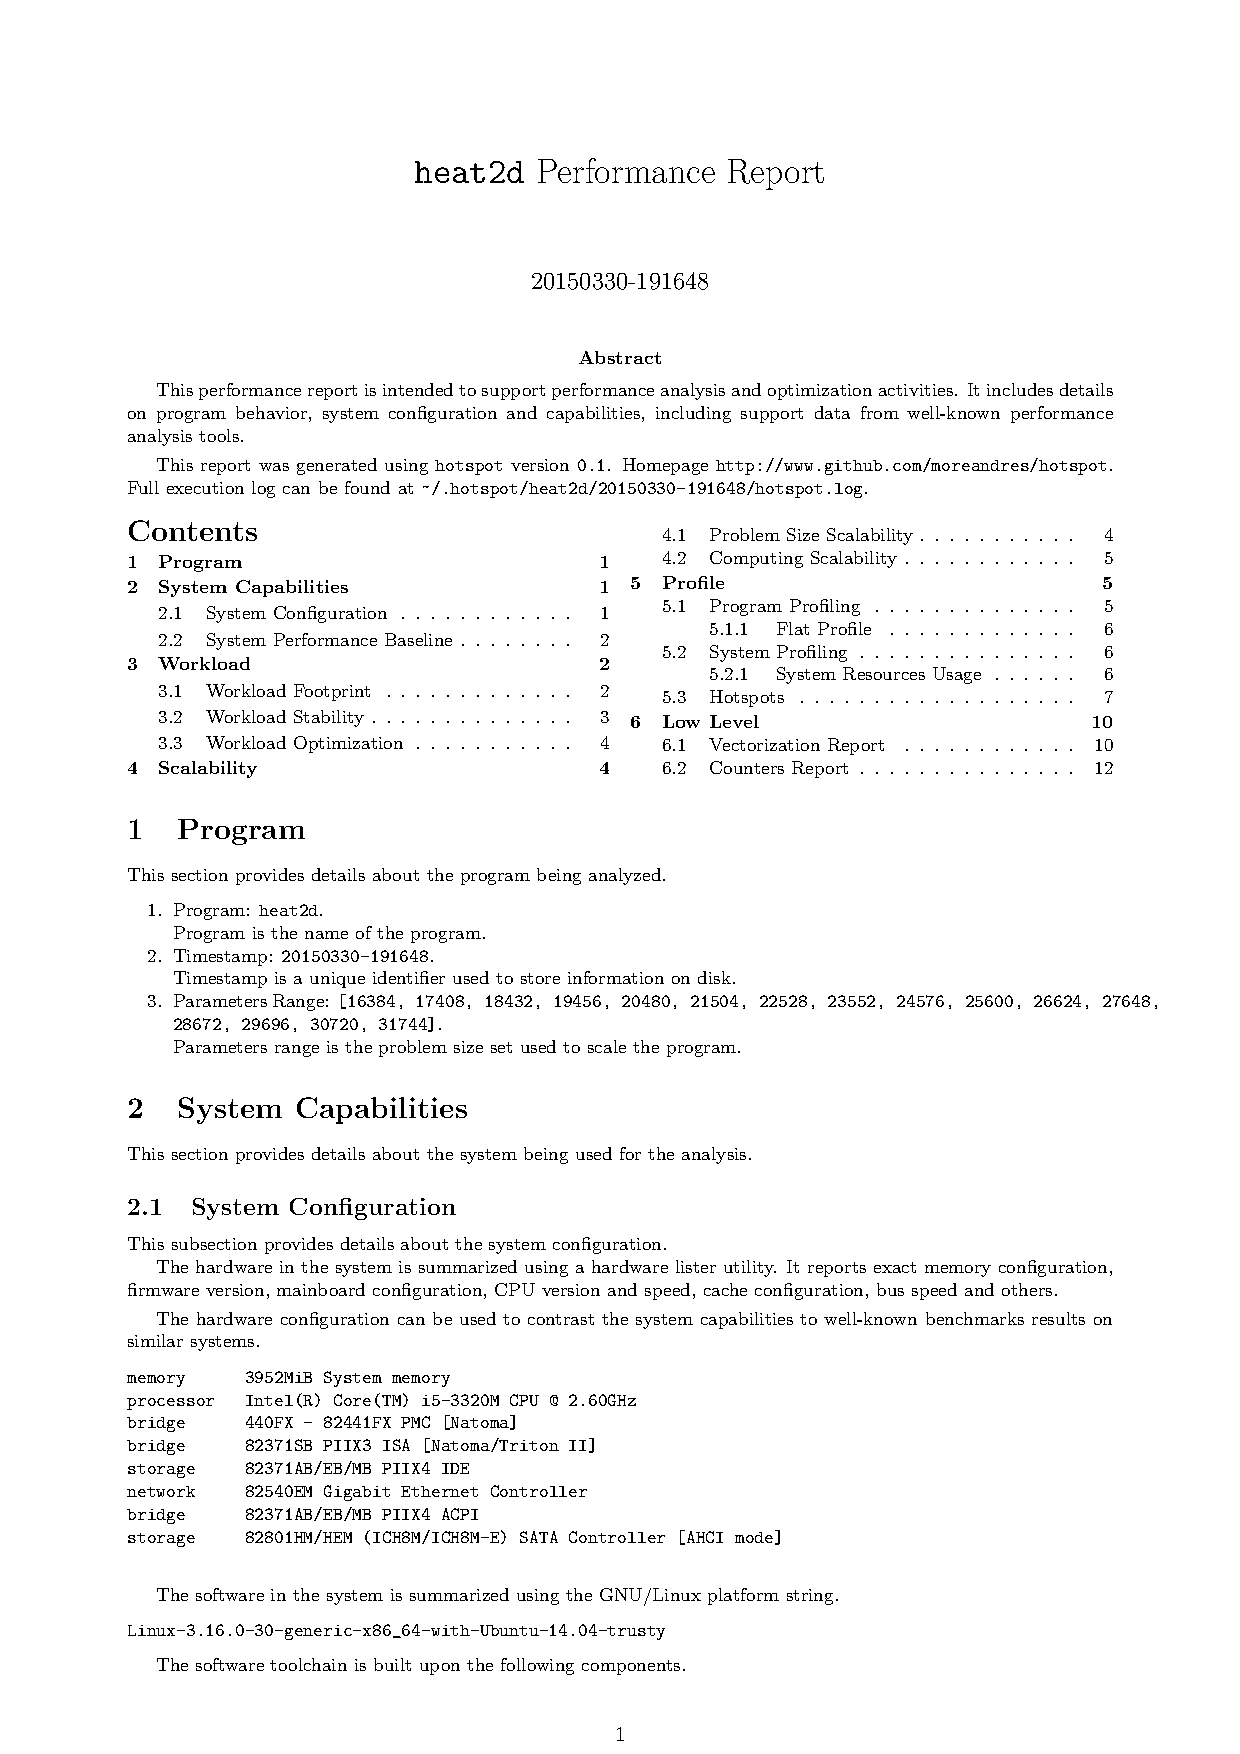
\includepdf[frame=true, pages=-, scale=0.75, pagecommand={}]{heat2d.pdf}

\section{Conjunto de Mandelbrot} \label{example-mandel}
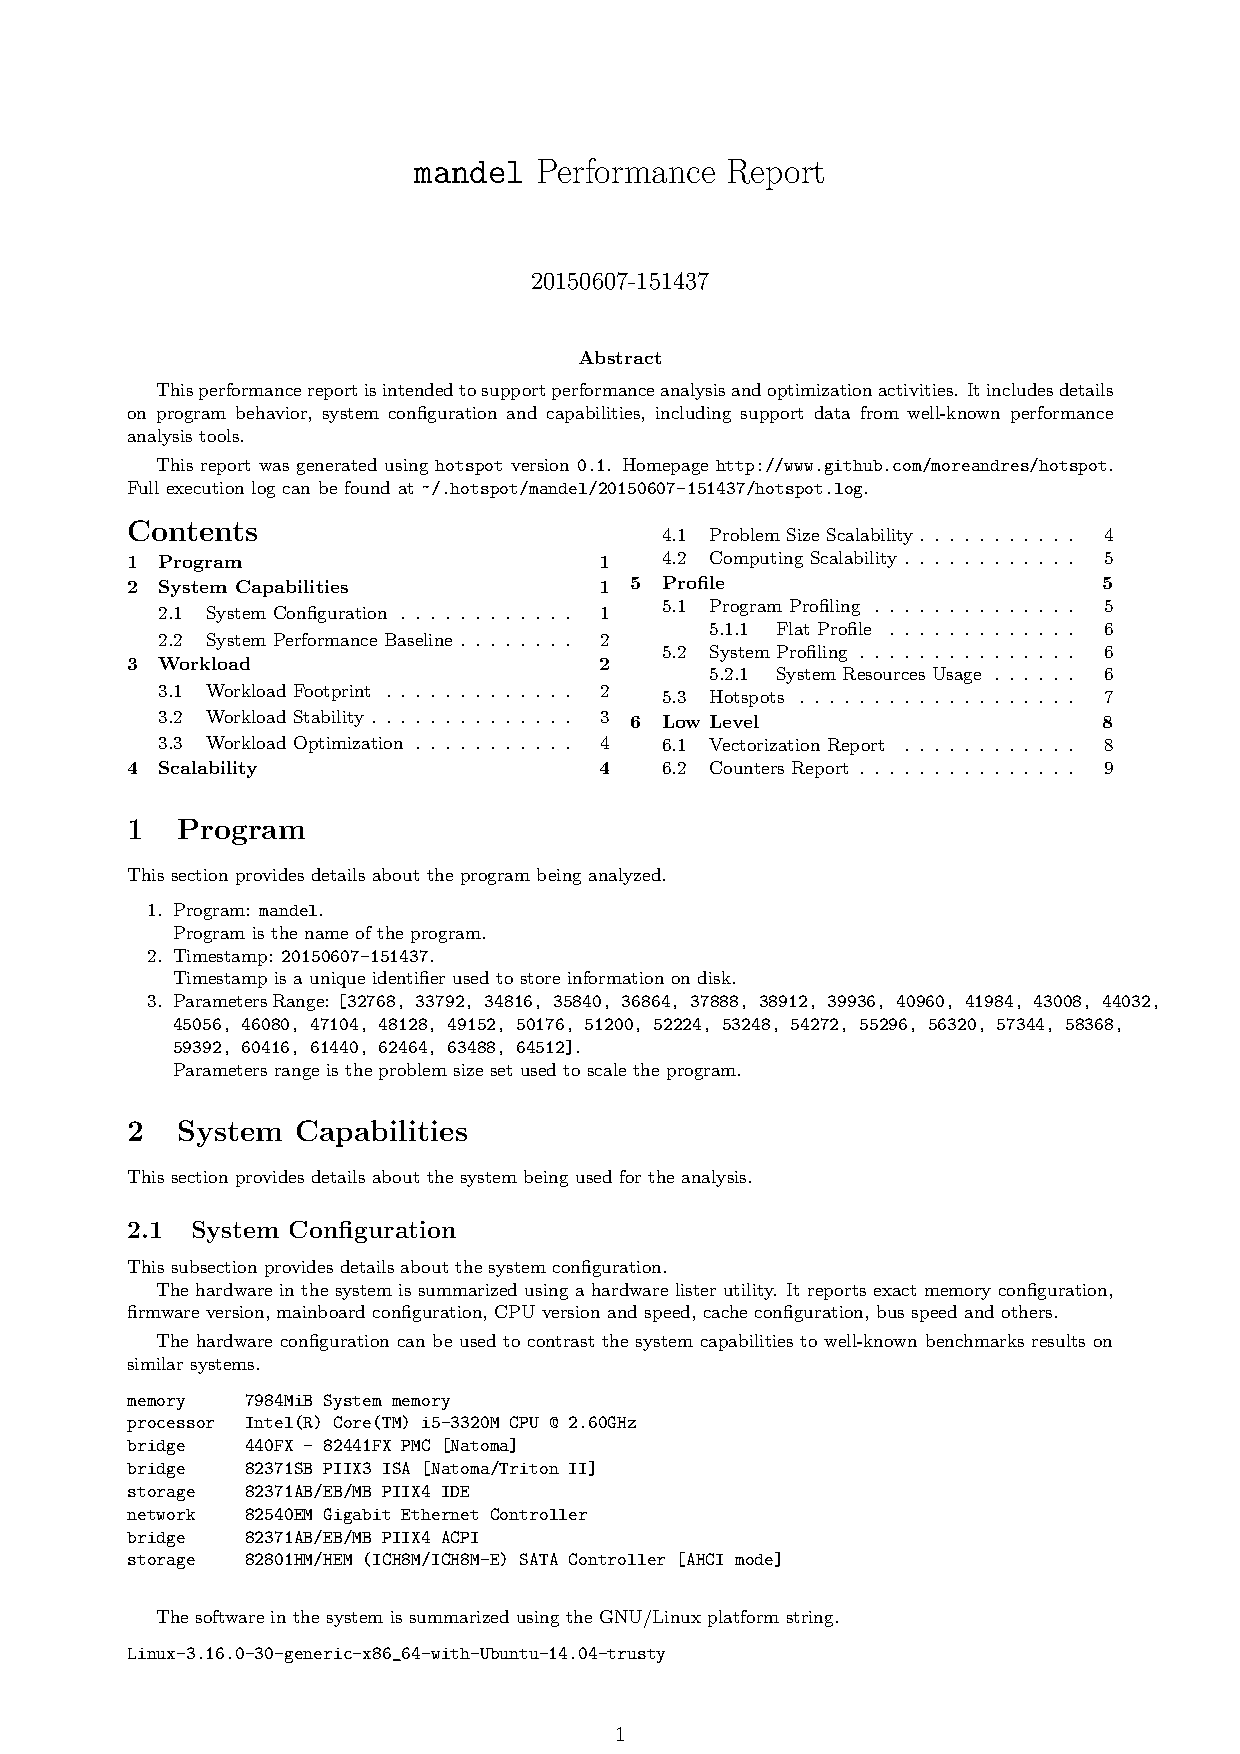
\includepdf[frame=true, pages=-, scale=0.75, pagecommand={}]{mandel.pdf}

\chapter{Contribuciones} \label{contributions}

\section{Reportes Técnicos}

\subsection{Estudio de Multiplicación de Matrices}

Estudio de Multiplicación de Matrices. Reporte Técnico. Realizado como parte del curso {\it Programación en Clusters} dictado por el Dr {\it Fernando Tinetti} \cite{mm-tool}.

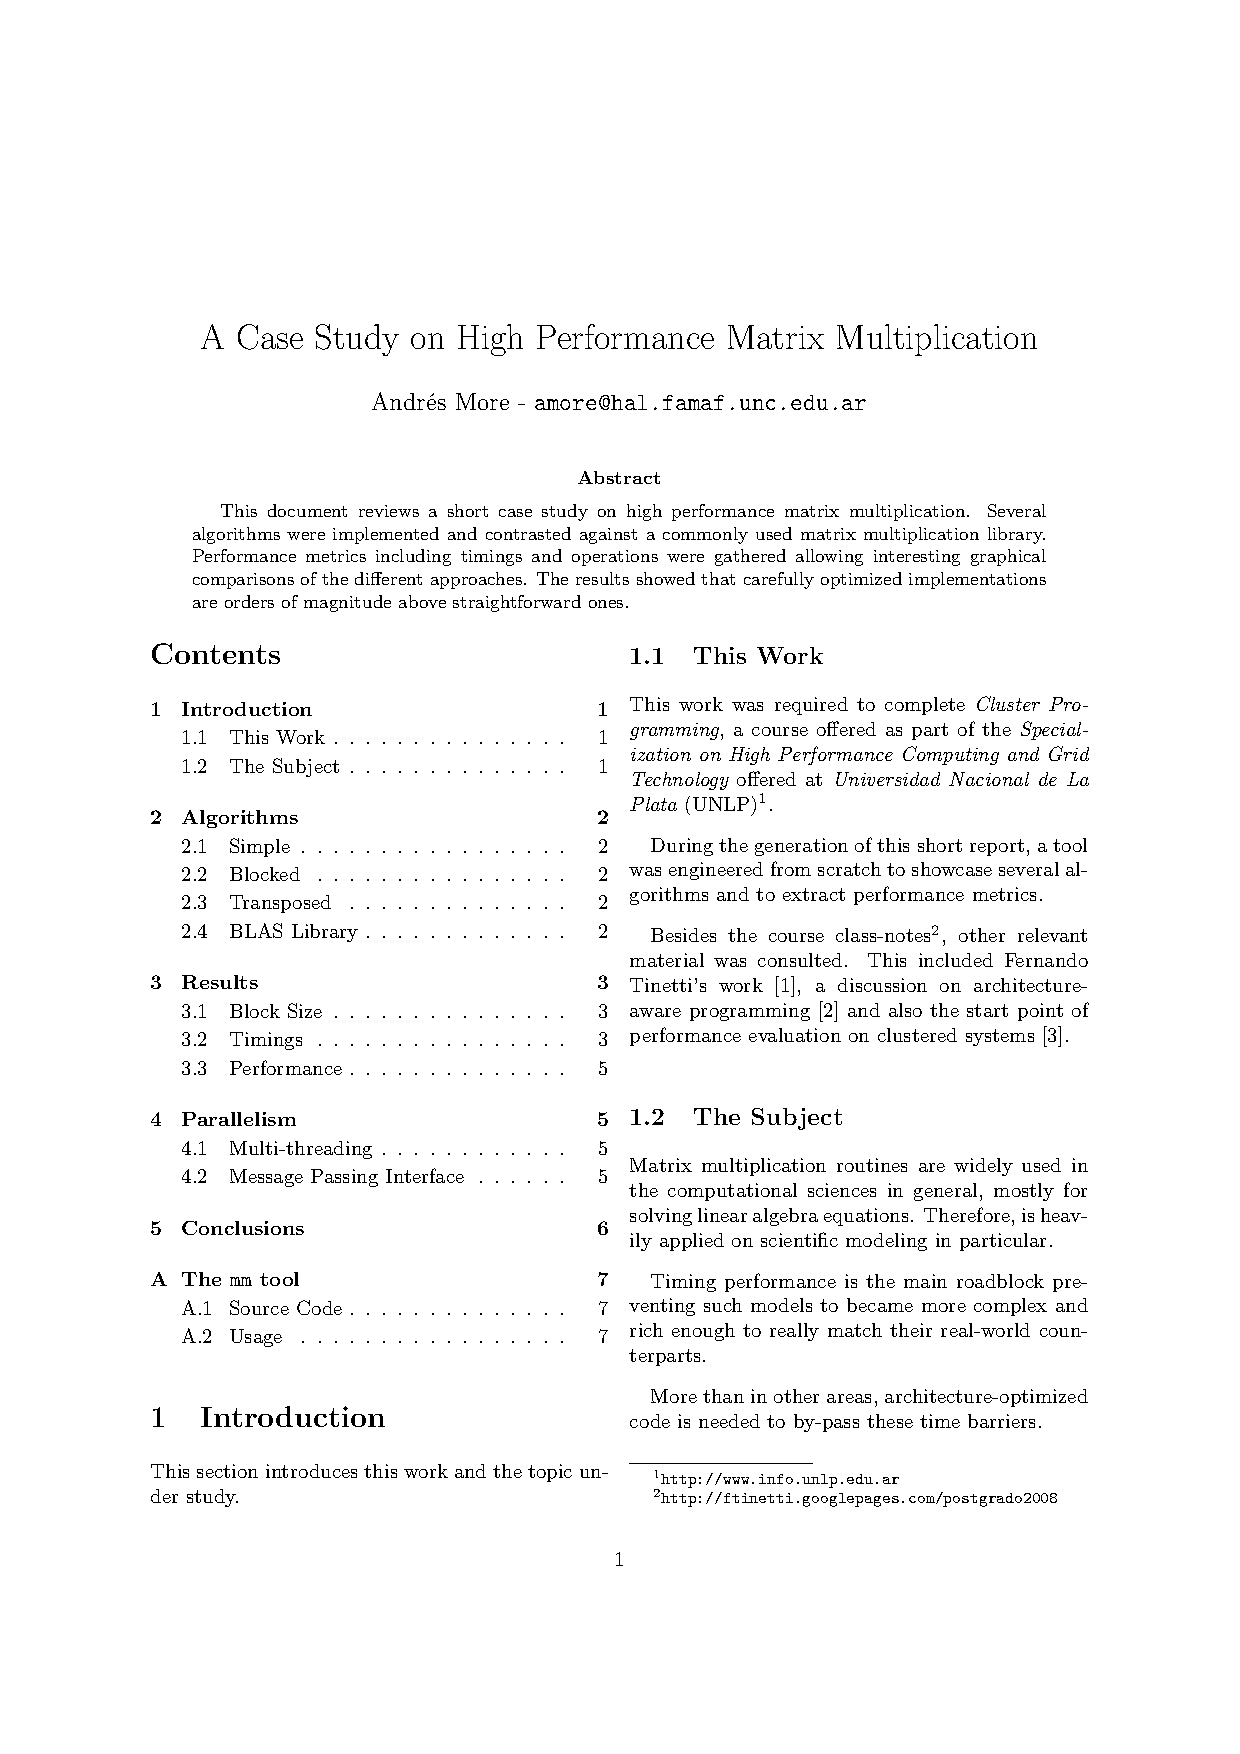
\includepdf[frame=true, pages=-, scale=0.75, pagecommand={}]{CaseStudyOnMatrixMultiplication.pdf}

\subsection{Comparación de Implementaciones de una Operación BLAS}

Comparación de Implementaciones de una Operación BLAS. Reporte técnico realizado como parte del curso {\it Programación GPU de Propósito General} dictado por la Dra {\it Margarita Amor}.

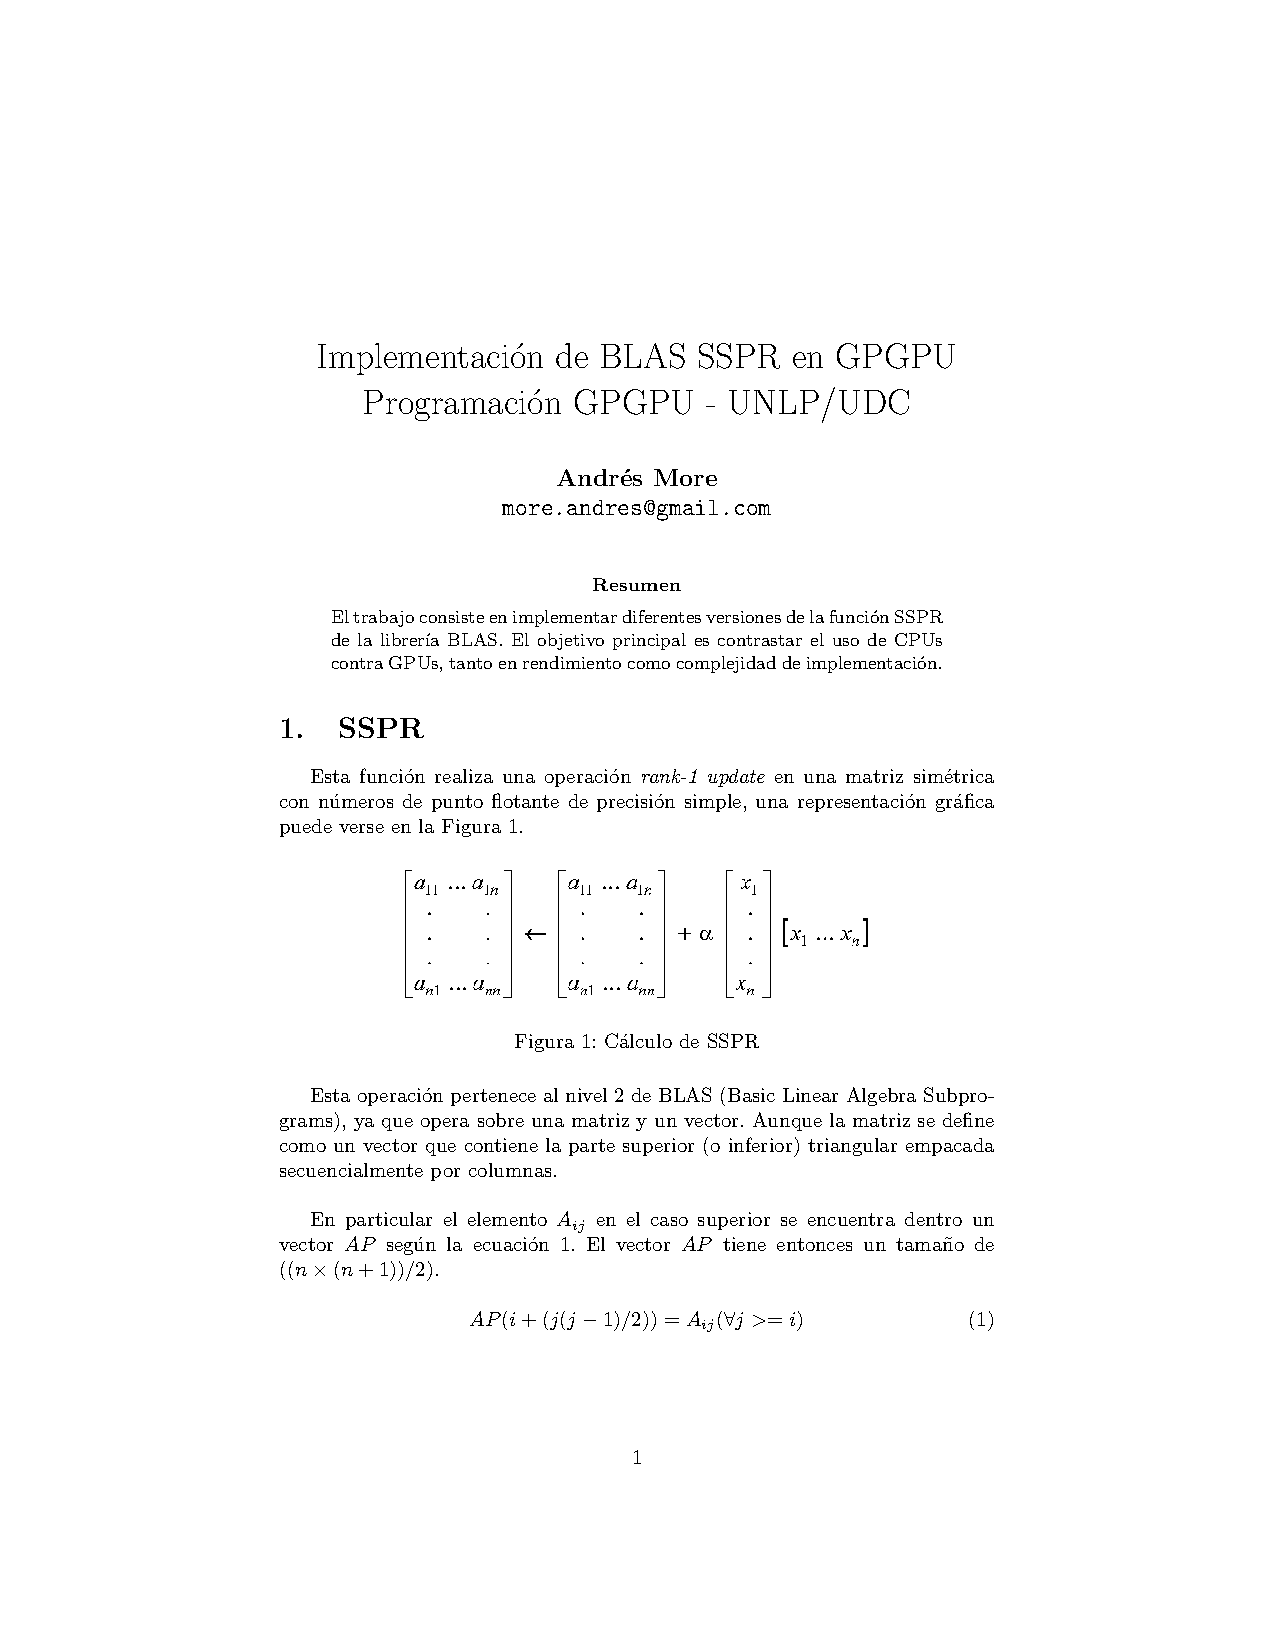
\includepdf[frame=true, pages=-, scale=0.75, pagecommand={}]{sspr.pdf}

\section{Artículos en Conferencias}

\subsection{\it Optimizing Latency in Beowulf Clusters}

Artículo {\it Optimizing Latency in Beowulf Clusters}. HPC Latam 2012 \cite{latency}.

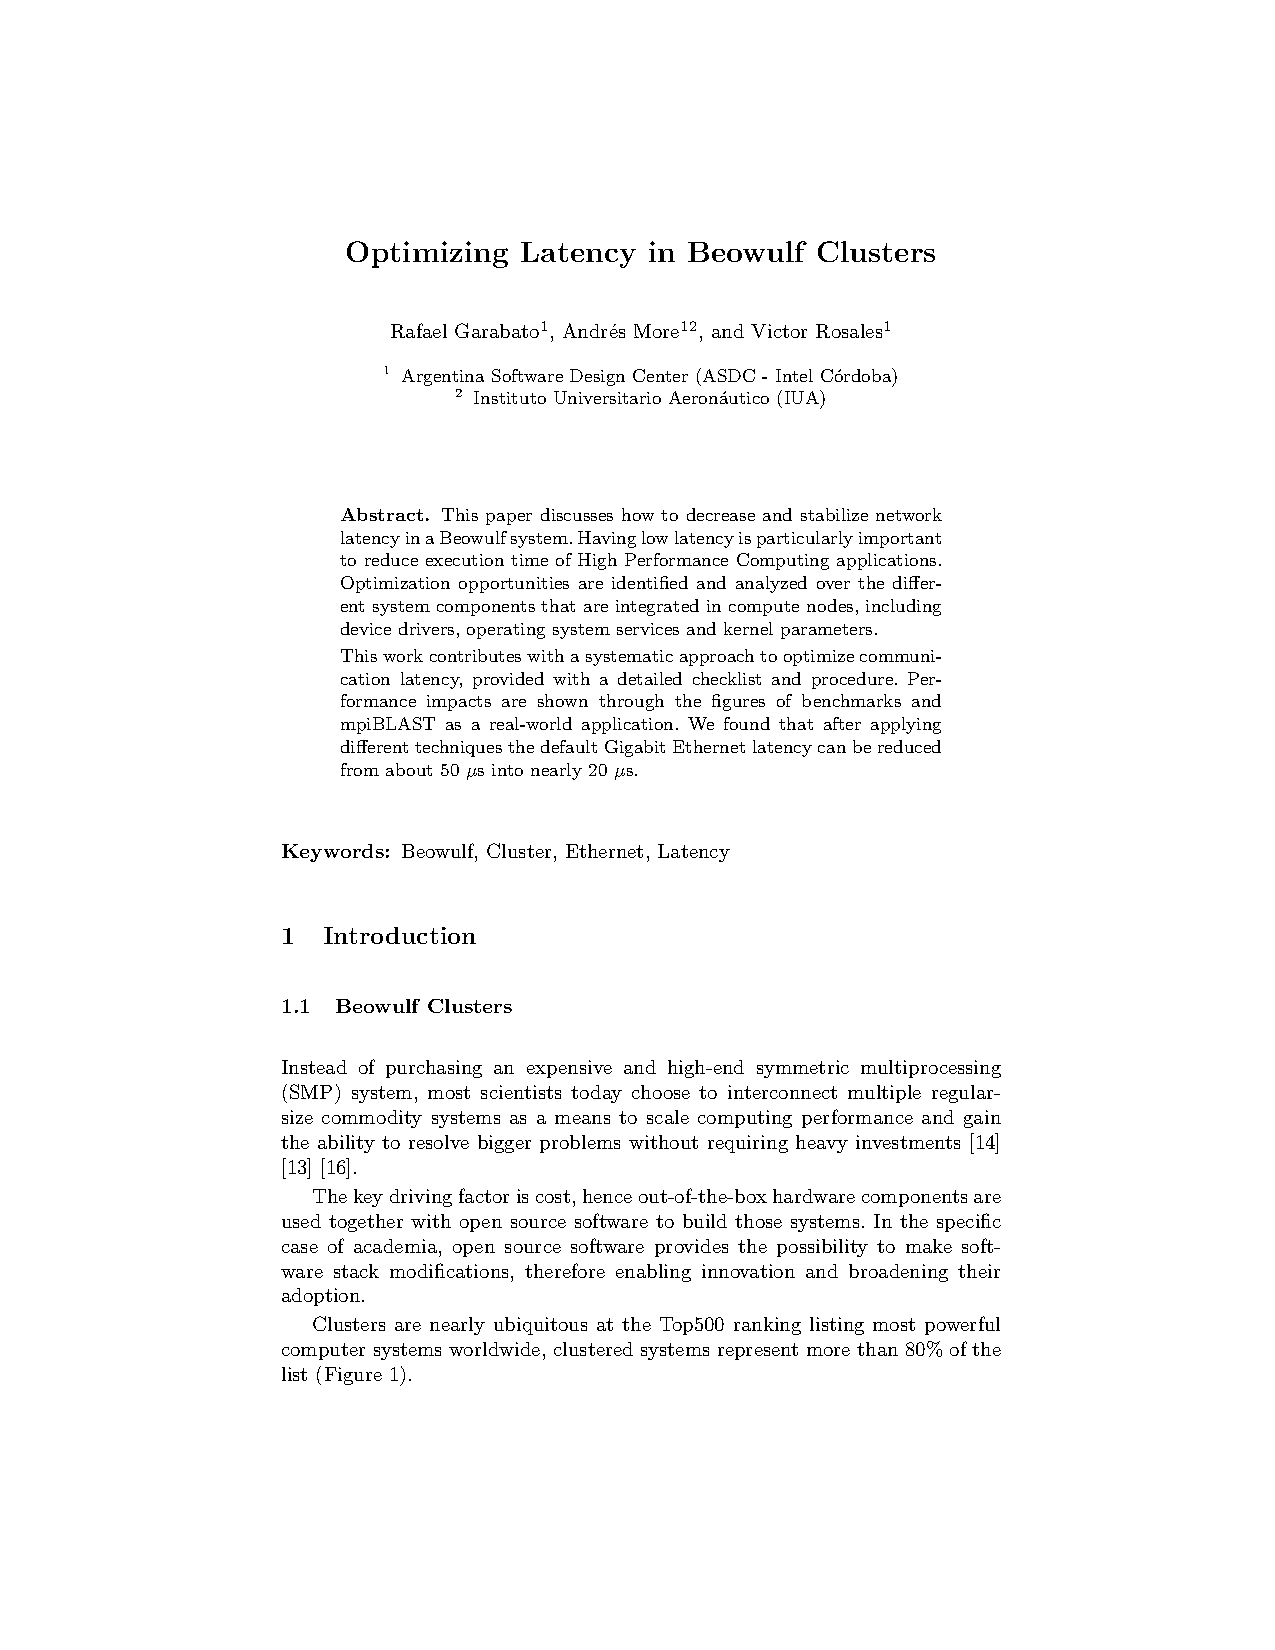
\includepdf[frame=true, pages=-, scale=0.75, pagecommand={}]{v15n3p03.pdf}

\section{{\it Lessons Learned from Contrasting BLAS Kernel Implementations}}

Artículo {\it Lessons Learned from Contrasting BLAS Kernel Implementations} - XIII Workshop Procesamiento Distribuido y Paralelo (WPDP), 2013 \cite{lessons}.

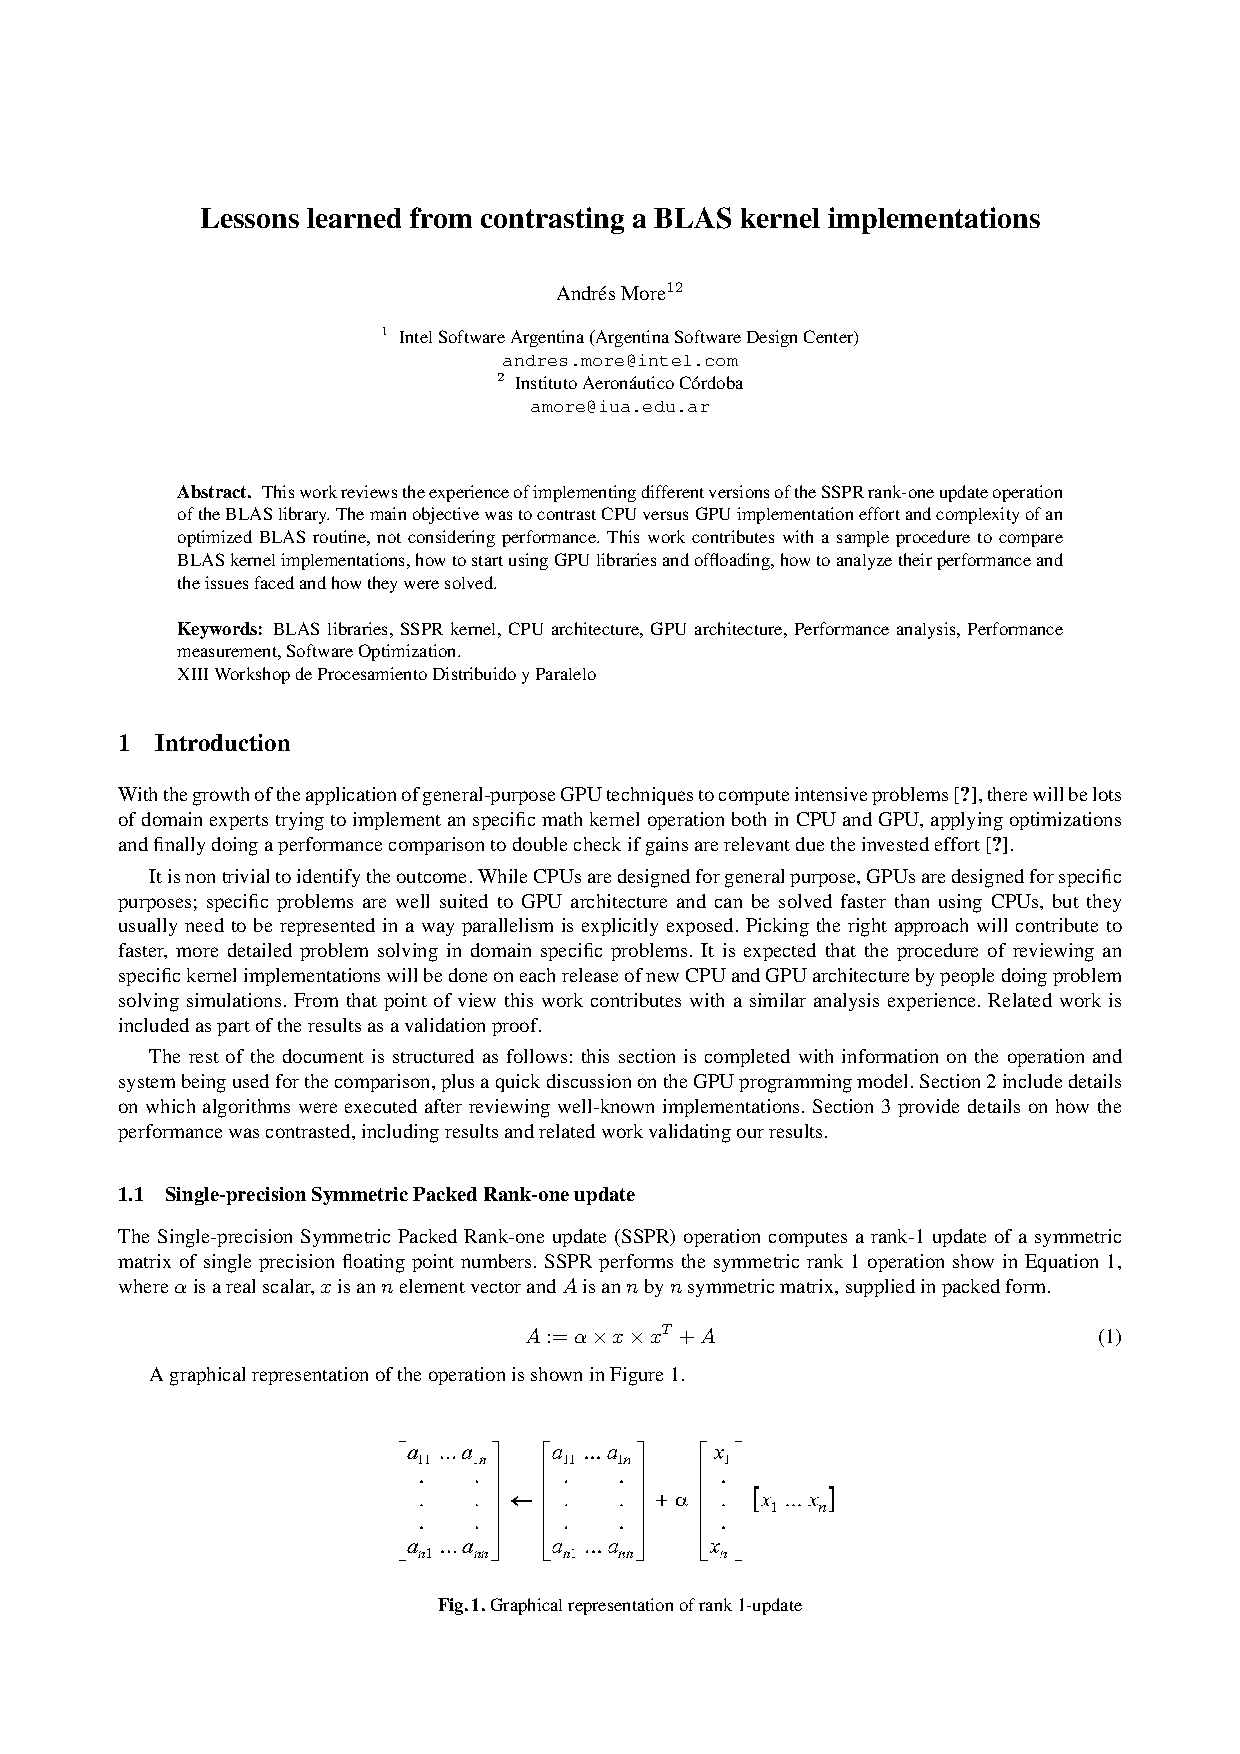
\includepdf[frame=true, pages=-, scale=0.75, pagecommand={}]{sspr-paper.pdf}

\section{Libros}

\subsection{Contribuciones en el Libro {\it Programming Intel Xeon Phi}}

Agradecimiento incluído de los autores por el borrador de los capítulos sobre {\it Intel Cluster Checker} e {\it Intel Cluster Ready}.

\section{Reseña del Libro {\it Intel Xeon Phi Coprocessor High Performance Programming}}

Reseña del Libro {\it Intel Xeon Phi Coprocessor High Performance Programming} - JCS\&T Vol 13 N 2 Octubre 2013 \footnote{\href{http://journal.info.unlp.edu.ar/journal/journal36/papers/JCST-Oct13-BR1.pdf}{JCS\&T Vol. 13 No. 2}}.

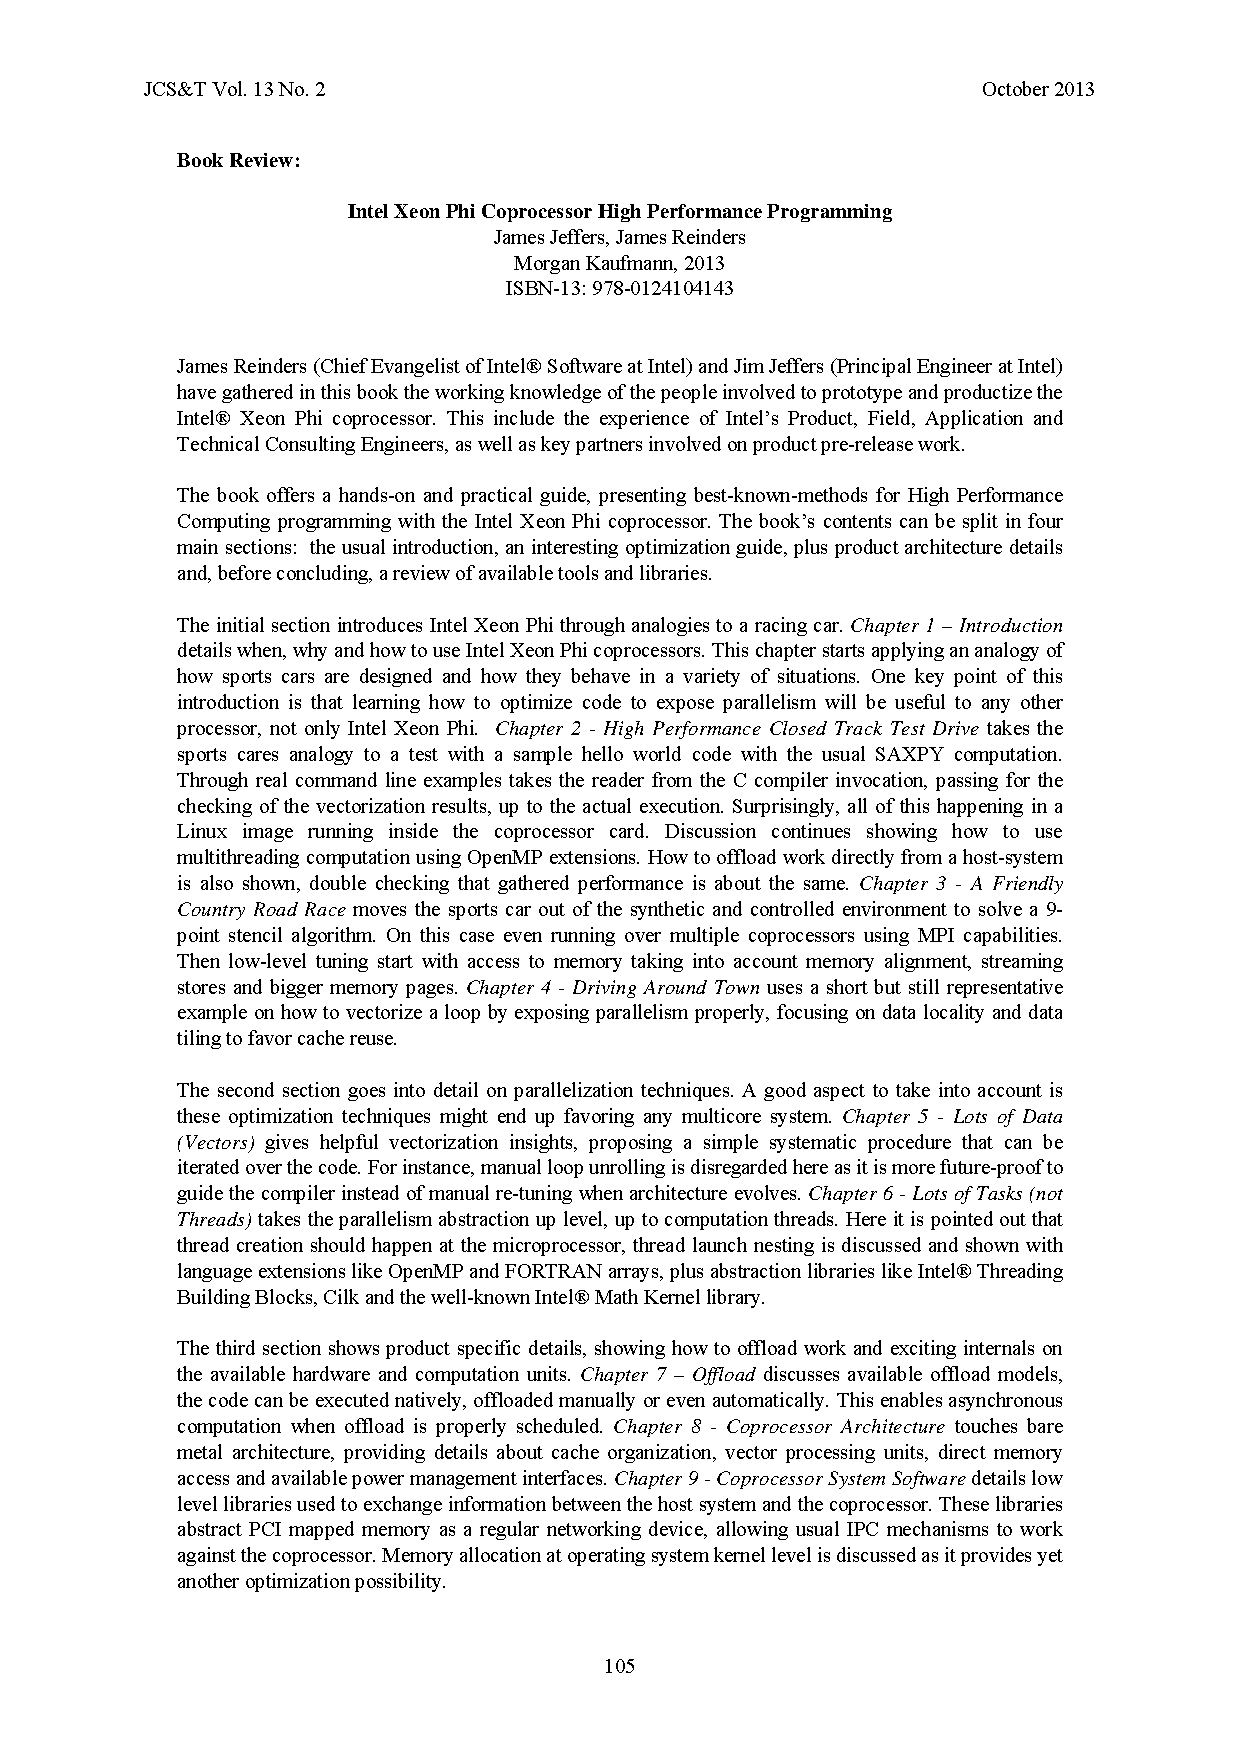
\includepdf[frame=true, pages=-, scale=0.75, pagecommand={}]{JCST-Oct13-BR1.pdf}

\end{document}
